\begin{frame}{Context -- Machine learning application}
    \begin{tikzpicture}[remember picture,overlay]
        \begin{scope}[xshift=0.5\textwidth]
            \node (problem) at (0,3.5) {\textbf{Tabular ML dataset}};
            %
            \node (table) at (0,1.5) {
                \begin{tabular}{c|cccc|c}
                    \toprule
                    & \textbf{Feature 1} & \textbf{Feature 2} & $\quad$...$\quad$ & \textbf{Feature n} & $\ \ $\textbf{Target}$\ \ $ \\
                    \midrule
                    \textbf{Sample 1} & \textcolor{mDarkTeal!20}{$a_{1,1}$} & \textcolor{mDarkTeal!20}{$a_{1,2}$} & \textcolor{mDarkTeal!20}{...} & \textcolor{mDarkTeal!20}{$a_{1,\pdim}$} & \textcolor{mDarkTeal!20}{$\obsi{1}$} \\
                    \textbf{Sample 2} & \textcolor{mDarkTeal!20}{$a_{2,1}$} & \textcolor{mDarkTeal!20}{$a_{2,2}$} & \textcolor{mDarkTeal!20}{...} & \textcolor{mDarkTeal!20}{$a_{2,\pdim}$} & \textcolor{mDarkTeal!20}{$\obsi{2}$} \\
                    \textbf{Sample 3} & \textcolor{mDarkTeal!20}{$a_{3,1}$} & \textcolor{mDarkTeal!20}{$a_{3,2}$} & \textcolor{mDarkTeal!20}{...} & \textcolor{mDarkTeal!20}{$a_{3,\pdim}$} & \textcolor{mDarkTeal!20}{$\obsi{3}$} \\
                    \textcolor{mDarkTeal!20}{...} & \textcolor{mDarkTeal!20}{...} & \textcolor{mDarkTeal!20}{...} & \textcolor{mDarkTeal!20}{...} & \textcolor{mDarkTeal!20}{...} & \textcolor{mDarkTeal!20}{...} \\
                    \textbf{Sample m} & \textcolor{mDarkTeal!20}{$a_{\ddim,1}$} & \textcolor{mDarkTeal!20}{$a_{\ddim,2}$} & \textcolor{mDarkTeal!20}{...} & \textcolor{mDarkTeal!20}{$a_{\ddim,\pdim}$} & \textcolor{mDarkTeal!20}{$\obsi{\ddim}$} \\
                    \bottomrule
                \end{tabular}
            };
            %
            \node[draw,ultra thick,fill=TolLightWhite,font=\small] (features) at ($(table.center)+(0,-0.5)$) {$\dic \in \kR^{\ddim\times\pdim}$};
            \node[draw,ultra thick,fill=TolLightWhite,font=\small] (outcome) at ($(table.center)+(4.2,-0.5)$) {$\obs \in \kR^{\ddim}$};
            %
            \node[text width=0.275\linewidth,align=center] (feature) at ($(table.south)+(-3.5,-0.6)$) {Features $\dic \in \kR^{\ddim\times\pdim}$};
            \node[text width=0.275\linewidth,align=center] (outcome) at ($(table.south)+(3.5,-0.6)$) {Target $\obs = \phi(\dic\pv)$};
            %
            \draw[ultra thick,<->] (feature) -- (outcome) node[midway,below] {weights $\pv \in \kR^{\pdim}$};
            %
            \node[font=\small,text width=0.3\linewidth,align=center] (loss) at ($(table.south)+(-1.75,-2)$) {\textbf{Model accuracy} \\ Loss $\mathcal{L}_{\phi}(\dic\pv,\obs)$};
            %
            \node[font=\small,text width=0.3\linewidth,align=center] (reg) at ($(table.south)+(1.75,-2)$) {\textbf{Model explicability} \\ Sparsity-inducing $\mathcal{R}(\pv)$};
            %
            \draw[ultra thick,->] (loss) -- ($(loss)+(0,-0.75)$);
            \draw[ultra thick,->] (reg) -- ($(reg)+(0,-0.75)$);
            %
            \node[align=center,text width=0.45\textwidth] (serm) at ($(table.south)+(0,-3.25)$) {
            \begin{blockcolor}{mDarkTeal}{Optimization problem}
                    \centering
                    $\min_{\pv \in \kR^{\pdim}} \mathcal{L}_{\phi}(\dic\pv,\obs) + \reg\mathcal{R}(\pv)$
                \end{blockcolor}
            };
        \end{scope}
    \end{tikzpicture}
\end{frame}

\begin{frame}{Context -- Algebra application}
    \begin{tikzpicture}[remember picture,overlay]
        \begin{scope}[xshift=0.5\textwidth]
            \onslide<1->{
                \node at (0,3.5) {\textbf{Sparse Component Analysis}};
                %
                \node[align=center,text width=0.675\textwidth] (goal) at (-2,1) {
                    \begin{blockcolor}{mDarkTeal}{Goal}
                        \centering
                        Given $\mathbf{M} \in \kR^{\ddim\times\pdim}$, find $\mathbf{D} \in \kR^{\ddim\times r}$ and $\mathbf{B} \in \kR^{r\times\pdim}$ such that $\textcolor{TolLightOrange}{\mathbf{M} \simeq \mathbf{D}\mathbf{B}}$ with \textcolor{TolLightOrange}{sparse} columns in $\mathbf{B}$.
                    \end{blockcolor}
                };
                %
                \node[align=center,text width=0.675\textwidth] (problem) at (-2,-1) {
                    \begin{blockcolor}{mDarkTeal}{Optimization problem}
                        \centering
                        $\min_{\mathbf{D} \in \kR^{\ddim\times r}, \mathbf{B} \in \kR^{r\times\pdim}} \tfrac{1}{2}\norm{\mathbf{M} - \mathbf{D}\mathbf{B}}{F}^2 + \reg\sum_{\idxentry=1}^{\pdim}\norm{\mathbf{b}_{\idxentry}}{0}$
                    \end{blockcolor}
                };
                %
                \draw[ultra thick,->] (-2,0.05) -- (-2,-0.45);
            }
            %
            %
            %
            \onslide<2->{
                \node[xshift=110] (0,0) {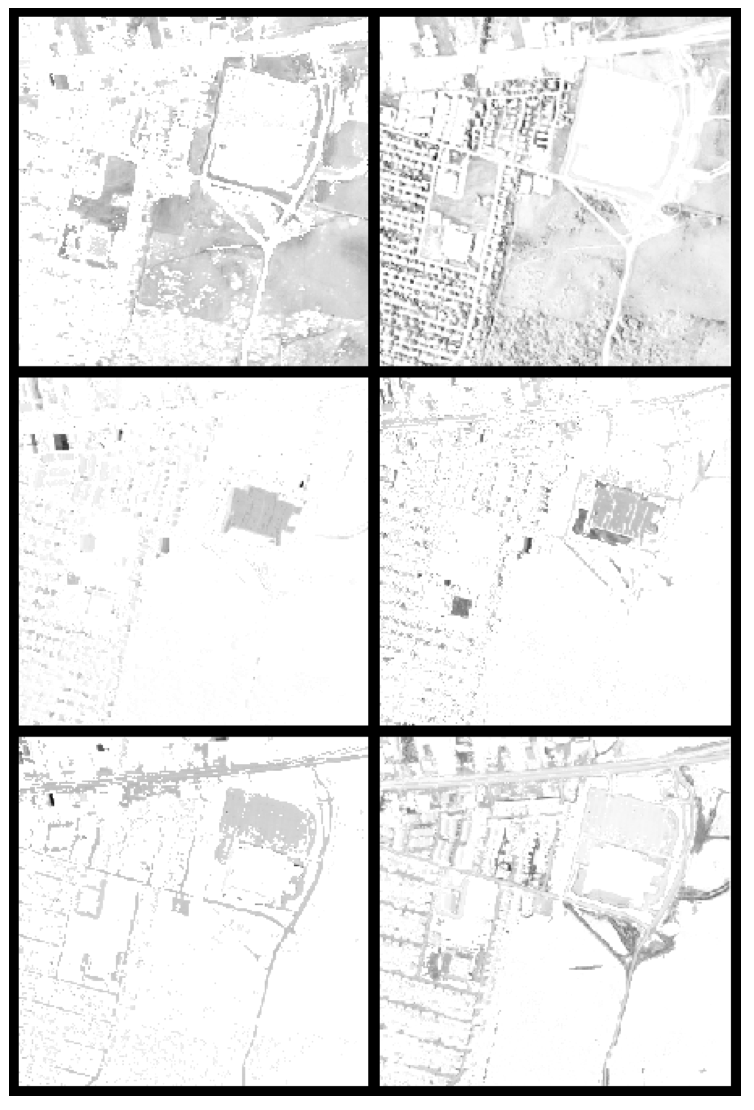
\includegraphics[width=3.5cm]{img/sca.png}};
                \node[xshift=110,font=\small] at (0,2.75) {J. Cohen, N. Gillis (2019)};
                \node[xshift=110,font=\small,text width=0.3\linewidth,align=center] at (0,-3.25) {Extract material abundance map from hyperspectral image};
            }
        \end{scope}
    \end{tikzpicture}
\end{frame}

\begin{frame}{Context -- Operation research application}
    \begin{tikzpicture}

        % Define the coordinates of the nodes for reuse
        \coordinate (A) at (0,0);
        \coordinate (B) at (2,0);
        \coordinate (C) at (1,2);
        \coordinate (D) at (1,-2);
        \coordinate (E) at (3,1);
        \coordinate (F) at (3,-1);
        \coordinate (G) at (-1,1.5);
        \coordinate (H) at (-1,-1.5);
        \coordinate (I) at (4,0);
        \coordinate (J) at (-2,0);
      
        % Draw the first pane with nodes only
        \begin{scope}[scale=0.75]
          \node[ultra thick, circle, draw, minimum size=6mm] (A) at (0,0) {};
          \node[ultra thick, circle, draw, minimum size=6mm] (B) at (2,0) {};
          \node[ultra thick, circle, draw, minimum size=6mm, TolLightRed] (C) at (1,2) {\small\textcolor{TolLightRed}{\textbf{3}}};
          \node[ultra thick, circle, draw, minimum size=6mm, TolLightRed] (D) at (1,-2) {\small\textcolor{TolLightRed}{\textbf{3}}};
          \node[ultra thick, circle, draw, minimum size=6mm] (E) at (3,1) {};
          \node[ultra thick, circle, draw, minimum size=6mm] (F) at (3,-1) {};
          \node[ultra thick, circle, draw, minimum size=6mm] (G) at (-1,1.5) {};
          \node[ultra thick, circle, draw, minimum size=6mm] (H) at (-1,-1.5) {};
          \node[ultra thick, circle, draw, minimum size=6mm, TolLightRed] (I) at (4,0) {\small\textcolor{TolLightRed}{\textbf{3}}};
          \node[ultra thick, circle, draw, minimum size=6mm, TolLightBlue] (J) at (-2,0) {};
    
          \draw[ultra thick] (A) -- (B);
          \draw[ultra thick] (A) -- (C);
          \draw[ultra thick] (A) -- (D);
          \draw[ultra thick] (A) -- (G);
          \draw[ultra thick] (A) -- (H);
          \draw[ultra thick] (B) -- (C);
          \draw[ultra thick] (B) -- (D);
          \draw[ultra thick] (B) -- (E);
          \draw[ultra thick] (B) -- (F);
          \draw[ultra thick] (B) -- (I);
          \draw[ultra thick] (C) -- (E);
          \draw[ultra thick] (C) -- (G);
          \draw[ultra thick] (D) -- (F);
          \draw[ultra thick] (D) -- (H);
          \draw[ultra thick] (E) -- (I);
          \draw[ultra thick] (F) -- (I);
          \draw[ultra thick] (G) -- (H);
          \draw[ultra thick] (G) -- (J);
          \draw[ultra thick] (H) -- (J);
          \draw[ultra thick] (I) -- (E);
    
          \node[text width=0.5\linewidth,align=center] at (1,3.5) {Max. capacity per edge: 10 \\ Edge construction cost: 5};
          \node[text width=0.5\linewidth,align=center] at (1,-3.5) {Which edges to build to transport flows from \textcolor{TolLightBlue}{source} to \textcolor{TolLightRed}{sink} nodes ?};

          \node[text width=0.35\linewidth,align=center] at (9,1) {
            \begin{blockcolor}{mDarkTeal}{Network design}
                \centering
                $\textstyle
                \left\{
                    \begin{array}{rl}
                        \min & Q(\pv) + \reg\norm{\pv}{0} \\ 
                        \text{s.t.} & \mathbf{D}\pv \leq \mathbf{d}, \ \pv \leq \mathbf{c} \\ & \pv \in \kR+^{\card(E)}
                    \end{array}
                \right.$
            \end{blockcolor}
          };
          \node[text width=0.5\linewidth,align=left] at (10.5,-2) {\begin{itemize}[nosep]\item[$Q$ :] transportation cost \item[$\reg$ :] unit construction cost \item[$\mathbf{D}\pv \leq \mathbf{d}$ :] flow conservation \item[$\pv \leq \mathbf{c}$ :] capacity constraint\end{itemize}};
        \end{scope}
    \end{tikzpicture}
\end{frame}

\begin{frame}{Context -- Signal processing application}
    \begin{tikzpicture}[remember picture,overlay]
        \begin{scope}[xshift=0.5\textwidth]
            \node at (0,3.5) {\textbf{Compressive sensing}};
            %
            \node[text width=0.25\linewidth,align=center] (groundtruth) at (-4,2.5) {Sparse signal \\ $\pv \in \kR^{\pdim}$};
            \node[text width=0.25\linewidth,align=center] (observation) at (4,2.5) {Observation \\ $\obs = \dic\pv + \boldsymbol{\epsilon} \in \kR^{\ddim}$};
            %
            \draw[ultra thick,->] ($(groundtruth.north east)+(0,-0.25)$) .. controls (0,3.25) .. ($(observation.north west)+(0,-0.25)$) node[midway,fill=TolLightWhite,draw,ultra thick,text width=0.35\linewidth,align=center,yshift=-5] {Linear measurement};
            \draw[ultra thick,<-] ($(groundtruth.south east)+(0,0.25)$) .. controls (0,1.75) .. ($(observation.south west)+(0,0.25)$) node[midway,fill=TolLightWhite,draw,ultra thick,text width=0.35\linewidth,align=center,yshift=5] {Recover $\pv$ from $\dic$ and $\obs$};
            %
            \draw ($(groundtruth)+(0,-1.75)$) node {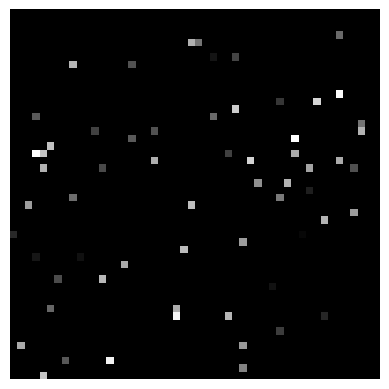
\includegraphics[width=2cm]{img/cs-x.png}};
            \draw ($(observation)+(0,-1.75)$) node {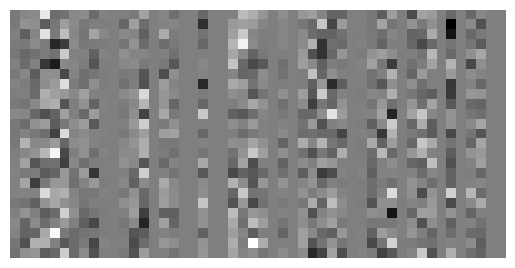
\includegraphics[width=2.5cm]{img/cs-y.png}};
            %
            \node [text width=0.45\textwidth] at (-3,-1) (problem) {
                \begin{blockcolor}{mDarkTeal}{Goal}
                    \centering
                    Find $\pv$ such that $\obs \simeq \dic\pv$
                \end{blockcolor}
            }; 
            %
            \node [text width=0.45\textwidth] at ($(problem)+(0,-2.25)$) (problem-sparse) {
                \begin{blockcolor}{mDarkTeal}{Goal (with sparse prior)}
                    \centering
                    Find $\pv$ \textcolor{TolLightOrange}{sparse} such that $\obs \simeq \dic\pv$
                \end{blockcolor}
            };
            %
            \draw[ultra thick,->] ($(problem)+(0,-0.75)$) -- ($(problem-sparse)+(0,0.5)$) node[midway,fill=TolLightWhite,draw,ultra thick] {$\ddim \ll \pdim$ : no unique solution};
            %
            \node [text width=0.45\textwidth] at (3,-1) (problem) {
                \begin{blockcolor}{mDarkTeal}{Optimization problem}
                    \centering
                    $\min_{\pv \in \kR^{\pdim}} \tfrac{1}{2}\norm{\obs - \dic\pv}{2}^2$
                \end{blockcolor}
            }; 
            %
            \node [text width=0.45\textwidth] at ($(problem)+(0,-2.25)$) (problem-sparse) {
                \begin{blockcolor}{mDarkTeal}{Sparse optimization problem}
                    \centering
                    $\min_{\pv \in \kR^{\pdim}} \tfrac{1}{2}\norm{\obs - \dic\pv}{2}^2 + \textcolor{TolLightOrange}{\reg\norm{\pv}{0}}$
                \end{blockcolor}
            };
            %
            \draw[ultra thick,->] ($(problem)+(0,-0.75)$) -- ($(problem-sparse)+(0,0.5)$) node[midway,fill=TolLightWhite,draw,ultra thick] {sparsity-inducing function};
        \end{scope}
    \end{tikzpicture}
\end{frame}

\begin{frame}{Context -- Balancing solution quality and problem hardness}
    \begin{tikzpicture}[remember picture,overlay]
        \begin{scope}[xshift=0.5\textwidth]
            \node (dataset) at (0,2.5) {
                \scriptsize
                \begin{tabular}{c|cccccc|c}
                    \multicolumn{8}{c}{\small{Riboflavin dataset - P. Bühlmann \textit{et al.} (2014)}} \\
                    \toprule
                    Colony & AADK & AAPA & ABFA & ABH & ... & ZUR & \textbf{B2 prod.} \\
                    \midrule
                    \#1 & 8.49 & 8.11 & 8.32 & 10.28 & ... & 7.42 & \textbf{-6.64} \\
                    \#2 & 7.29 & 6.39 & 11.32 & 9.42 & ... & 6.99 & \textbf{-5.43} \\
                    ... & ... & ... & ... & ... & ... & ... & ... \\
                    \#71 & 6.85 & 8.27 & 7.98 & 8.04 & ... & 6.65 & \textbf{-7.58} \\
                    \bottomrule
                \end{tabular}
            };
            %
            \draw[ultra thick,-] ($(dataset.south)+(-2.4,0)$) -- ($(dataset.south)+(-2.4,-0.05)$) -- ($(dataset.south)+(2.15,-0.05)$) node[midway,below,font=\small] {4,088 genes} -- ($(dataset.south)+(2.15,0)$);
        \end{scope}
        %
        \begin{scope}[xshift=30,yshift=-80]
            \pgfplotscreateplotcyclelist{cycle_quality_hardness}{
                TolLightBlue, very thick, mark=*, mark options={scale=0.5}\\
                TolLightGreen, very thick, mark=*, mark options={scale=0.5}\\
                TolLightBrown, very thick, mark=*, mark options={scale=0.5}\\    
                TolLightRed, very thick, mark=*, mark options={scale=0.5}\\
            }
            \begin{groupplot}[
                group style={
                    group size=2 by 1,
                    horizontal sep=0.2\textwidth,
                },
                width   = 0.48\textwidth,
                height  = 0.4\textwidth,
                xlabel  = \textbf{Num. of genes},
                legend columns=5, 
                legend style={
                    at={(-0.35,1)},
                    anchor=south,
                    /tikz/every even column/.style = {column sep=5pt},
                    draw=none,
                },
                cycle list name=cycle_quality_hardness,
                mbaseplot,
                axis line style = ultra thick,
                major tick style = {ultra thick,color=mDarkTeal},
                minor tick style={draw=none},
                xmajorgrids=true,
                ymajorgrids=true,
                major grid style={dotted},
                axis x line=bottom,
                axis y line=left,
            ]

                \nextgroupplot[
                    ylabel = \textbf{Model error},
                    ymode=log,
                    ymin=0.09,
                    ymax=1.5,
                ]
                \foreach \method in {omp,lasso,enet,el0ps} {
                    \addplot table[x=nnz_grid,y=\method_test_error,col sep=comma]{data/riboflavin_quality.csv};
                }

                \nextgroupplot[
                    ymode=log,
                    ylabel = \textbf{Time (sec.)},
                    ytick={0.001,0.01,0.1,1,10,100},
                    ymax=70,
                    ymin=0.0004,
                ]
                \foreach \method in {omp,lasso,enet,el0ps} {
                    \addplot table[x=nnz_grid,y=\method_solve_time,col sep=comma]{data/riboflavin_quality.csv};
                }

                \addlegendentry{Omp (sklearn)};
                \addlegendentry{Lasso (sklearn)};
                \addlegendentry{E-Net (sklearn)};
                \addlegendentry{$\ell_0$-prob. (el0ps)};
            \end{groupplot}
        \end{scope}
    \end{tikzpicture}
\end{frame}

\begin{frame}{Context -- Balancing solution quality and problem hardness}
    \begin{tikzpicture}[remember picture,overlay]
        \begin{scope}[xshift=0.5\textwidth]
            \node[text width=0.25\linewidth,align=center] (groundtruth) at (-5,2.75) {Sparse signal \\ $\pv \in \kR^{\pdim}$};
            \node[text width=0.25\linewidth,align=center] (observation) at (-1,2.75) {Observation \\ $\obs = \dic\pv + \boldsymbol{\epsilon} \in \kR^{\ddim}$};
            %
            \draw[ultra thick,->] ($(groundtruth.north east)+(0,-0.25)$) .. controls (-3,3.5) .. ($(observation.north west)+(0,-0.25)$);
            \draw[ultra thick,<-] ($(groundtruth.south east)+(0,0.25)$) .. controls (-3,2) .. ($(observation.south west)+(0,0.25)$);
            %
            \node[text width=0.6\linewidth,align=center,font=\small] at (-3,1) {\textbf{Setup} \\ $\dic \in \kR^{100\times200}$ highly correlated, $\boldsymbol{\epsilon} \sim \mathcal{N}(0,\sigma\mathbf{I})$, \\ $\pv$ with 10 unit spikes of random location};
        \end{scope}
        %
        \begin{scope}[xshift=205,yshift=30]
            \pgfplotscreateplotcyclelist{cycle_quality_hardness}{
                TolLightBlue, very thick, mark=*, mark options={scale=0.5}\\
                TolLightGreen, very thick, mark=*, mark options={scale=0.5}\\
                TolLightBrown, very thick, mark=*, mark options={scale=0.5}\\    
                TolLightRed, very thick, mark=*, mark options={scale=0.5}\\
            }
            \begin{groupplot}[
                group style={
                    group size=1 by 1,
                    horizontal sep=0.2\textwidth,
                },
                width   = 0.48\textwidth,
                height  = 0.4\textwidth,
                xlabel  = \textbf{Num. of non-zeros},
                legend columns=5, 
                legend style={
                    at={(-0.35,1)},
                    anchor=south,
                    /tikz/every even column/.style = {column sep=5pt},
                    draw=none,
                },
                cycle list name=cycle_quality_hardness,
                mbaseplot,
                axis line style = ultra thick,
                major tick style = {ultra thick,color=mDarkTeal},
                minor tick style={draw=none},
                xmajorgrids=true,
                ymajorgrids=true,
                major grid style={dotted},
                axis x line=bottom,
                axis y line=left,
            ]
                \nextgroupplot[
                    ylabel = \textbf{F1-score},
                    ymin=-0.1,
                    ymax=1.1,
                ]
                    \foreach \method in {omp,lasso,enet,proposed} {
                        \addplot table[x=nnz_grid,y=\method_f1_score,col sep=comma]{data/statistics_random_unit.csv};
                    }
            \end{groupplot}
        \end{scope}
        %
        \begin{scope}[xshift=25,yshift=-95]
            \pgfplotscreateplotcyclelist{cycle_quality_hardness}{
                TolLightBlue, very thick, mark=*, mark options={scale=0.5}\\
                TolLightGreen, very thick, mark=*, mark options={scale=0.5}\\
                TolLightBrown, very thick, mark=*, mark options={scale=0.5}\\    
                TolLightRed, very thick, mark=*, mark options={scale=0.5}\\
            }
            \begin{groupplot}[
                group style={
                    group size=2 by 1,
                    horizontal sep=0.25\textwidth,
                },
                width   = 0.48\textwidth,
                height  = 0.4\textwidth,
                xlabel  = \textbf{Num. of non-zeros},
                legend columns=5, 
                legend style={
                    at={(-0.35,1)},
                    anchor=south,
                    /tikz/every even column/.style = {column sep=5pt},
                    draw=none,
                },
                cycle list name=cycle_quality_hardness,
                mbaseplot,
                axis line style = ultra thick,
                major tick style = {ultra thick,color=mDarkTeal},
                minor tick style={draw=none},
                xmajorgrids=true,
                ymajorgrids=true,
                major grid style={dotted},
                axis x line=bottom,
                axis y line=left,
            ]

                \nextgroupplot[
                    ylabel = \textbf{Model error},
                    ymode=log,
                    ymin=0.09,
                    ymax=1.5,
                ]
                \foreach \method in {omp,lasso,enet,proposed} {
                    \addplot table[x=nnz_grid,y=\method_test_error,col sep=comma]{data/statistics_random_unit.csv};
                }

                \nextgroupplot[
                    ymode=log,
                    ylabel = \textbf{Time (sec.)},
                    ytick={0.001,0.01,0.1,1,10,100},
                    ymax=70,
                    ymin=0.0004,
                ]
                \foreach \method in {omp,lasso,enet,proposed} {
                    \addplot table[x=nnz_grid,y=\method_solve_time,col sep=comma]{data/statistics_random_unit.csv};
                }

                \addlegendentry{Omp (sklearn)};
                \addlegendentry{Lasso (sklearn)};
                \addlegendentry{E-Net (sklearn)};
                \addlegendentry{$\ell_0$-prob. (el0ps)};
            \end{groupplot}
        \end{scope}
    \end{tikzpicture}
\end{frame}

\begin{frame}{Context -- Balancing solution quality and problem hardness}
    \begin{tikzpicture}[remember picture,overlay]
        \begin{scope}[xshift=0.5\textwidth]
            \node[text width=0.25\linewidth,align=center] (groundtruth) at (-5,2.75) {Sparse signal \\ $\pv \in \kR^{\pdim}$};
            \node[text width=0.25\linewidth,align=center] (observation) at (-1,2.75) {Observation \\ $\obs = \dic\pv + \boldsymbol{\epsilon} \in \kR^{\ddim}$};
            %
            \draw[ultra thick,->] ($(groundtruth.north east)+(0,-0.25)$) .. controls (-3,3.5) .. ($(observation.north west)+(0,-0.25)$);
            \draw[ultra thick,<-] ($(groundtruth.south east)+(0,0.25)$) .. controls (-3,2) .. ($(observation.south west)+(0,0.25)$);
            %
            \node[text width=0.6\linewidth,align=center,font=\small] at (-3,1) {\textbf{Setup} \\ $\dic \in \kR^{100\times200}$ highly correlated, $\boldsymbol{\epsilon} \sim \mathcal{N}(0,\sigma\mathbf{I})$, \\ $\pv$ with 10 unit and evenly-spaced spikes};
        \end{scope}
        %
        \begin{scope}[xshift=205,yshift=30]
            \pgfplotscreateplotcyclelist{cycle_quality_hardness}{
                TolLightBlue, very thick, mark=*, mark options={scale=0.5}\\
                TolLightGreen, very thick, mark=*, mark options={scale=0.5}\\
                TolLightBrown, very thick, mark=*, mark options={scale=0.5}\\    
                TolLightRed, very thick, mark=*, mark options={scale=0.5}\\
            }
            \begin{groupplot}[
                group style={
                    group size=1 by 1,
                    horizontal sep=0.2\textwidth,
                },
                width   = 0.48\textwidth,
                height  = 0.4\textwidth,
                xlabel  = \textbf{Num. of non-zeros},
                legend columns=5, 
                legend style={
                    at={(-0.35,1)},
                    anchor=south,
                    /tikz/every even column/.style = {column sep=5pt},
                    draw=none,
                },
                cycle list name=cycle_quality_hardness,
                mbaseplot,
                axis line style = ultra thick,
                major tick style = {ultra thick,color=mDarkTeal},
                minor tick style={draw=none},
                xmajorgrids=true,
                ymajorgrids=true,
                major grid style={dotted},
                axis x line=bottom,
                axis y line=left,
            ]
                \nextgroupplot[
                    ylabel = \textbf{F1-score},
                    ymin=-0.1,
                    ymax=1.1,
                ]
                    \foreach \method in {omp,lasso,enet,proposed} {
                        \addplot table[x=nnz_grid,y=\method_f1_score,col sep=comma]{data/statistics_2outof3_unit.csv};
                    }
            \end{groupplot}
        \end{scope}
        %
        \begin{scope}[xshift=25,yshift=-95]
            \pgfplotscreateplotcyclelist{cycle_quality_hardness}{
                TolLightBlue, very thick, mark=*, mark options={scale=0.5}\\
                TolLightGreen, very thick, mark=*, mark options={scale=0.5}\\
                TolLightBrown, very thick, mark=*, mark options={scale=0.5}\\    
                TolLightRed, very thick, mark=*, mark options={scale=0.5}\\
            }
            \begin{groupplot}[
                group style={
                    group size=2 by 1,
                    horizontal sep=0.25\textwidth,
                },
                width   = 0.48\textwidth,
                height  = 0.4\textwidth,
                xlabel  = \textbf{Num. of non-zeros},
                legend columns=5, 
                legend style={
                    at={(-0.35,1)},
                    anchor=south,
                    /tikz/every even column/.style = {column sep=5pt},
                    draw=none,
                },
                cycle list name=cycle_quality_hardness,
                mbaseplot,
                axis line style = ultra thick,
                major tick style = {ultra thick,color=mDarkTeal},
                minor tick style={draw=none},
                xmajorgrids=true,
                ymajorgrids=true,
                major grid style={dotted},
                axis x line=bottom,
                axis y line=left,
            ]

                \nextgroupplot[
                    ylabel = \textbf{Model error},
                    ymode=log,
                    ymin=0.09,
                    ymax=1.5,
                ]
                \foreach \method in {omp,lasso,enet,proposed} {
                    \addplot table[x=nnz_grid,y=\method_test_error,col sep=comma]{data/statistics_2outof3_unit.csv};
                }

                \nextgroupplot[
                    ymode=log,
                    ylabel = \textbf{Time (sec.)},
                    ytick={0.001,0.01,0.1,1,10,100},
                    ymax=70,
                    ymin=0.0004,
                ]
                \foreach \method in {omp,lasso,enet,proposed} {
                    \addplot table[x=nnz_grid,y=\method_solve_time,col sep=comma]{data/statistics_2outof3_unit.csv};
                }

                \addlegendentry{Omp (sklearn)};
                \addlegendentry{Lasso (sklearn)};
                \addlegendentry{E-Net (sklearn)};
                \addlegendentry{$\ell_0$-prob. (el0ps)};
            \end{groupplot}
        \end{scope}
    \end{tikzpicture}
\end{frame}

\begin{frame}{Context -- A bit of history}
    \begin{tikzpicture}[remember picture,overlay]
        \begin{scope}[xshift=0.5\textwidth]
            \node[align=center,text width=0.5\textwidth] (problem) at (0,3) {
                \begin{blockcolor}{mDarkTeal}{Problem}
                    \centering
                    $\min_{\pv \in \kR^{\pdim}} \lfunc(\dic\pv) + \reg\norm{\pv}{0} + \pfunc(\pv)$
                \end{blockcolor}
            };
            %
            \node (linecenter) at ($(current page.north)+(0,-0.5\textheight)$) {};
            \draw [ultra thick,->] ($(linecenter)+(-6,0)$) -- ($(linecenter)+(6,0)$) node (arrow) [midway] {};
            %
            \node (date1) at ($(linecenter)+(-5,0)$) {};
            \draw [ultra thick,-] ($(date1)+(0,-0.02\textheight)$) -- ($(date1)+(0,0.02\textheight)$);
            \node at ($(date1)+(0,+0.06\textheight)$)  {\textbf{1995}};
            \node[text width=0.2\textwidth,align=center,font=\small] at ($(date1)+(0,-0.05\textheight)$) {Heuristics};
            \node[text width=0.3\textwidth,align=center,font=\scriptsize] at ($(date1)+(0,-0.12\textheight)$) {MP, OMP, ... \\ S. Mallat (1993)};
            %
            \node (origin1) at ($(date1)+(0,-0.4\textheight)$) {};
            \fill[draw,thick,fill=TolLightWhite] ($(origin1)+(-0.5,0)$) circle (0.1);
            \fill[draw,thick,fill=TolLightOrange] ($(origin1)+(-0.5,0.3)$) circle (0.1);
            \fill[draw,thick,fill=TolLightWhite] ($(origin1)+(-0.5,0.6)$) circle (0.1);
            \fill[draw,thick,fill=TolLightWhite] ($(origin1)+(-0.5,0.9)$) circle (0.1);
            \fill[draw,thick,fill=TolLightWhite] ($(origin1)+(-0.5,1.2)$) circle (0.1);
            \fill[draw,thick,fill=TolLightWhite] ($(origin1)+(-0.5,1.5)$) circle (0.1);
            \node at ($(origin1)+(-0.5,-0.4)$) {$\pv^1$};
            %
            \fill[draw,thick,fill=TolLightWhite] ($(origin1)+(0,0)$) circle (0.1);
            \fill[draw,thick,fill=TolLightOrange] ($(origin1)+(0,0.3)$) circle (0.1);
            \fill[draw,thick,fill=TolLightWhite] ($(origin1)+(0,0.6)$) circle (0.1);
            \fill[draw,thick,fill=TolLightOrange] ($(origin1)+(0,0.9)$) circle (0.1);
            \fill[draw,thick,fill=TolLightWhite] ($(origin1)+(0,1.2)$) circle (0.1);
            \fill[draw,thick,fill=TolLightWhite] ($(origin1)+(0,1.5)$) circle (0.1);
            \node at ($(origin1)+(0,-0.4)$) {$\pv^2$};
            %
            \fill[draw,thick,fill=TolLightWhite] ($(origin1)+(0.5,0)$) circle (0.1);
            \fill[draw,thick,fill=TolLightOrange] ($(origin1)+(0.5,0.3)$) circle (0.1);
            \fill[draw,thick,fill=TolLightWhite] ($(origin1)+(0.5,0.6)$) circle (0.1);
            \fill[draw,thick,fill=TolLightOrange] ($(origin1)+(0.5,0.9)$) circle (0.1);
            \fill[draw,thick,fill=TolLightOrange] ($(origin1)+(0.5,1.2)$) circle (0.1);
            \fill[draw,thick,fill=TolLightWhite] ($(origin1)+(0.5,1.5)$) circle (0.1);
            \node at ($(origin1)+(0.5,-0.4)$) {$\pv^3$};
            %
            %
            %
            \node (date2) at ($(linecenter)+(-2.5,0)$) {};
            \draw [ultra thick,-] ($(date2)+(0,-0.02\textheight)$) -- ($(date2)+(0,0.02\textheight)$);
            \node at ($(date2)+(0,+0.06\textheight)$)  {\textbf{2000}};
            \node[text width=0.25\textwidth,align=center,font=\small] at ($(date2)+(0,-0.053\textheight)$) {Recovery cond.};
            \node[text width=0.3\textwidth,align=center,font=\scriptsize] at ($(date2)+(0,-0.12\textheight)$) {RIP, NSP, ... \\ E. Candes (2004)};
            %
            \node (origin2) at ($(date2)+(0,-0.4\textheight)$) {};
            \node[text width=0.2\linewidth,align=center] at ($(origin2)+(0,0.05\textheight)$) {OMP solves $\ell_0$-problem under RIP};
            %
            %
            %
            \node (date3) at ($(linecenter)+(0,0)$) {};
            \draw [ultra thick,-] ($(date3)+(0,-0.02\textheight)$) -- ($(date3)+(0,0.02\textheight)$);
            \node at ($(date3)+(0,+0.06\textheight)$)  {\textbf{2005}};
            \node[font=\small] at ($(date3)+(0,-0.053\textheight)$) {Convex approx.};
            \node[text width=0.3\textwidth,align=center,font=\scriptsize] at ($(date3)+(0,-0.12\textheight)$) {Lasso, Elastic-Net, ... \\ R. Tibshirani (2005)};
            %
            \node (origin3) at ($(date3)+(0,-0.4\textheight)$) {};
            \draw[ultra thick,->] ($(origin3)+(-1,0)$) -- ($(origin3)+(1, 0)$);
            \draw[ultra thick,->] ($(origin3)+(0,0)$) -- ($(origin3)+(0,1.5)$);
            \draw[-,very thick,TolLightOrange] ($(origin3)+(-0.05,0.8)$) -- ($(origin3)+(-1,0.8)$);
            \draw[-,very thick,TolLightOrange] ($(origin3)+(0.05,0.8)$) -- ($(origin3)+(1,0.8)$);
            \draw[very thick,dashed,TolLightOrange] (origin3) .. controls ($(origin3)+(-0.5,0.1)$) ..  ($(origin3)+(-1,0.8)$);
            \draw[very thick,dashed,TolLightOrange] (origin3) .. controls ($(origin3)+(0.5,0.1)$) ..  ($(origin3)+(1,0.8)$);
            \draw[TolLightOrange,very thick] ($(origin3)+(0,0.8)$) circle (0.075);
            \fill[TolLightOrange] (origin3) circle (0.075);
            %
            %
            %
            \node (date4) at ($(linecenter)+(2.5,0)$) {};
            \draw [ultra thick,-] ($(date4)+(0,-0.02\textheight)$) -- ($(date4)+(0,0.02\textheight)$);
            \node at ($(date4)+(0,+0.06\textheight)$)  {\textbf{2010}};
            \node[font=\small] at ($(date4)+(0,-0.053\textheight)$) {Concave approx.};
            \node[text width=0.3\textwidth,align=center,font=\scriptsize] at ($(date4)+(0,-0.12\textheight)$) {SCAD, MCP, ... \\ C. Zhang (2010)};
            %
            \node (origin4) at ($(date4)+(0,-0.4\textheight)$) {};
            \draw[ultra thick,->] ($(origin4)+(-1,0)$) -- ($(origin4)+(1, 0)$);
            \draw[ultra thick,->] ($(origin4)+(0,0)$) -- ($(origin4)+(0,1.5)$);
            \draw[-,very thick,TolLightOrange] ($(origin4)+(-0.05,0.8)$) -- ($(origin4)+(-1,0.8)$);
            \draw[-,very thick,TolLightOrange] ($(origin4)+(0.05,0.8)$) -- ($(origin4)+(1,0.8)$);
            \draw[very thick,TolLightOrange,dashed] (origin4) .. controls ($(origin4)+(-0.5,0.8)$) ..  ($(origin4)+(-1,0.8)$);
            \draw[very thick,TolLightOrange,dashed] (origin4) .. controls ($(origin4)+(0.5,0.8)$) ..  ($(origin4)+(1,0.8)$);
            \draw[TolLightOrange,very thick] ($(origin4)+(0,0.8)$) circle (0.075);
            \fill[TolLightOrange] (origin4) circle (0.075);
            %
            %
            %
            \node (date5) at ($(linecenter)+(5,0)$) {};
            \draw[ultra thick,-] ($(date5)+(0,-0.02\textheight)$) -- ($(date5)+(0,0.02\textheight)$);
            \node at ($(date5)+(0,+0.06\textheight)$)  {\textbf{2015}};
            \node[text width=0.22\textwidth,align=center,font=\small,TolLightOrange] at ($(date5)+(0,-0.05\textheight)$) {Exact methods};
            \node[text width=0.3\textwidth,align=center,font=\scriptsize] at ($(date5)+(0,-0.12\textheight)$) {MIP, BnB, ... \\ D. Bertsimas (2016)};
            %
            \node (origin5) at ($(date5)+(0,-0.4\textheight)$) {};
            \draw[ultra thick,->] ($(origin5)+(-1,0)$) -- ($(origin5)+(1, 0)$);
            \draw[ultra thick,->] ($(origin5)+(0,0)$) -- ($(origin5)+(0,1.5)$);
            \draw[-,very thick,TolLightOrange] ($(origin5)+(-0.05,0.8)$) -- ($(origin5)+(-1,0.8)$);
            \draw[-,very thick,TolLightOrange] ($(origin5)+(0.05,0.8)$) -- ($(origin5)+(1,0.8)$);
            \draw[TolLightOrange,very thick] ($(origin5)+(0,0.8)$) circle (0.075);
            \fill[TolLightOrange] (origin5) circle (0.075);
        \end{scope}
    \end{tikzpicture}
\end{frame}

\begin{frame}{Context -- MIP formulation}
    \begin{tikzpicture}[remember picture,overlay]
        \begin{scope}[xshift=0.5\textwidth]
            \node[align=center,text width=0.5\textwidth] (problem) at (-2.5,3.25) {
                \begin{blockcolor}{mDarkTeal}{Problem}
                    \centering
                    $\min_{\pv \in \kR^{\pdim}} \lfunc(\dic\pv) + \reg\norm{\pv}{0} + \pfunc(\pv)$
                \end{blockcolor}
            };
            %
            \node[text width=0.5\linewidth,align=center,font=\small] at ($(problem)+(5.75,-0.15)$) {\textbf{Use generic MIP solvers} \\ Need standardized expressions \\ linear/quadratic/conic/...};
            %
            \node[align=center,text width=0.5\textwidth] (mip) at ($(problem)+(0,-2.9)$) {
                \begin{blockcolor}{mDarkTeal}{MIP formulation}
                    \centering
                    $\left\{\begin{array}{rcl}\min && \lfunc(\dic\pv) + \reg\textcolor{TolLightOrange}{\transp{\1}\bv} + \pfunc(\pv) \\
                    \text{s.t.} && \textcolor{TolLightOrange}{\pvi{\idxentry} = 0 \implies \bvi{\idxentry} = 0, \ \forall \idxentry} \\
                    && \pv \in \kR^{\pdim}, \ \bv \in \{0,1\}^{\pdim}\end{array}\right.$
                \end{blockcolor}
            };
            %
            \node[text width=0.4\linewidth,align=center,font=\small] at ($(mip)+(5.75,-0.15)$) {\textbf{Lifted formulation} \\ $\norm{\pv}{0}$ $=$ $\transp{\1}\bv$ \\ for all $\pv \in \kR^{\pdim}$ and $\bv \in \{0,1\}^{\pdim}$ \\ if $\pvi{\idxentry} = 0$ $\implies$ $\bvi{\idxentry} = 0, \ \forall \idxentry$};
            %
            \draw[ultra thick,->] (problem) -- ($(mip.north)+(0,-0.25)$) node[midway,font=\small,fill=TolLightWhite,draw,ultra thick] {linearize $\ell_0$-norm};
            %
            \node[align=center,text width=0.5\textwidth] (practical-mip) at ($(mip)+(0,-3.25)$) {
                \begin{blockcolor}{mDarkTeal}{Practical MIP formulation}
                    \centering
                    $\left\{\begin{array}{rcl}\min && \lfunc(\dic\pv) + \reg\transp{\1}\bv + \textcolor{TolLightOrange}{\pfunc_{\text{mip}}}(\pv,\bv) \\
                    \text{s.t.} && \pv \in \kR^{\pdim}, \ \bv \in \{0,1\}^{\pdim}\end{array}\right.$
                \end{blockcolor}
            };
            %
            \draw[ultra thick,->] (mip) -- ($(practical-mip.north)+(0,-0.25)$) node[midway,font=\small,fill=TolLightWhite,draw,ultra thick] {avoid logical cstr.};
            %
            \node[text width=0.5\linewidth,align=center,font=\small] at ($(practical-mip)+(5.75,-0.15)$) {
                \textbf{Construct $\pfunc_{\text{mip}}$ depending on $\pfunc$} \\ \begin{tabular}{c|c} $\pfunc(\pv)$ & $\pfunc_{\text{mip}}(\pv,\bv)$ \\ \toprule $\icvx(\norm{\pv}{\infty} \leq \bigM)$ & $\icvx(-\bigM\bv \leq \pv \leq \bigM\pv)$ \\ $\regtwo\norm{\pv}{2}^2$ & $\sum_{\idxentry=1}^{\pdim}\regtwo\tfrac{\pvi{\idxentry}^2}{\bvi{\idxentry}}$\end{tabular}
            };
        \end{scope}
    \end{tikzpicture}
\end{frame}

\begin{frame}{Context -- Research community}
    \begin{tikzpicture}[remember picture,overlay]
        \node[fill=TolLightOrange] at ($(current page.north)+(4.8,-1.3)$) {\textcolor{TolLightWhite}{Non-exhaustive list}};
        %
        \node[align=center,text width=0.3\linewidth] (usa) at ($(current page.center)+(-2.3,2)$) {
\includegraphics[width=1.5\textwidth]{img/usa.png}};
        %
        \draw[<-,ultra thick] ($(usa)+(1.9,-0.7)$) .. controls ($(usa)+(4.7,-0.4)$) .. ($(usa)+(5,0.1)$) node [above,align=center,font=\scriptsize] {\textbf{MIT}~\\ D. Bertsimas, R. Mazmuder, ...~\\\textit{MIO tools for $\ell_0$-problems}};
        %
        \draw[<-,ultra thick] ($(usa)+(0.25,0.45)$) .. controls ($(usa)+(-1.9,0.1)$) .. ($(usa)+(-2.3,-0.1)$) node [below,align=center,font=\scriptsize] {\textbf{Google Deep Mind}~\\ H. Hazimeh, A. Dedieu, ...~\\\textit{MIO-based heuristics and} \\ \textit{softwares}};
        %
        \draw[<-,ultra thick] ($(usa)+(-0.5,-1.2)$) .. controls ($(usa)+(-1.5,-1.4)$) .. ($(usa)+(-2,-1.9)$) node [below,align=center,font=\scriptsize] {\textbf{Berkley}~\\ A. Atamtürk, A. Gomès, ...~\\\textit{Convex-based acceleration}};
        %
        %
        %
        \node[align=center,text width=0.3\linewidth] (europe) at ($(current page.center)+(3.75,-2.5)$) {
\includegraphics[width=1.5\textwidth]{img/europe.png}};
        %
        \draw[<-,ultra thick] ($(europe)+(0.7,1)$) .. controls ($(europe)+(0.5,1.5)$) .. ($(europe)+(1.1,3.5)$) node [above,align=center,font=\scriptsize] {\textbf{Lund University}~\\ M. Carlsson, C. Olsson...~\\\textit{Quadratic envelope}};
        %
        \draw[<-,ultra thick] ($(europe)+(0.4,0.1)$) .. controls ($(europe)+(-0.5,1.5)$) .. ($(europe)+(-1.2,2.5)$) node [above,align=center,font=\scriptsize] {\textbf{Frankfurt / Wurzburg Universities}~\\ C. Kanzow, A. Tillmann, ...~\\\textit{Optimality conditions}};
        %
        \draw[<-,ultra thick] ($(europe)+(-0.4,0.5)$) .. controls ($(europe)+(-1,1.3)$) .. ($(europe)+(-2,1.5)$) node [above left,align=center,font=\scriptsize] {\textbf{London Business School}~\\ J. Pauphilet, R. Cory-Wright, ...~\\\textit{Healthcare applications}};
        %
        \draw[<-,ultra thick] ($(europe)+(0.2,-0.6)$) .. controls ($(europe)+(-1.5,0.8)$) .. ($(europe)+(-2.5,0.9)$) node [left,align=center,font=\scriptsize] {\textbf{Ponts ParisTech}~\\ M. De Lara, P. Chancelier, A. Parmentier, ...~\\\textit{Non-convex analysis for $\ell_0$-norm, ML appli.}};
        %
        \draw[<-,ultra thick] ($(europe)+(-0.4,-0.4)$) .. controls ($(europe)+(-1,-0.4)$) .. ($(europe)+(-5,-0.2)$) node [left,align=center,font=\scriptsize] {\textbf{Centrale Nantes / ENSTA Bretagne}~\\ S. Bourguignon, J. Ninin, ...~\\\textit{Branch-and-Bound for $\ell_0$-problems}};
        %
        \draw[<-,ultra thick] ($(europe)+(-0.2,-0.7)$) .. controls ($(europe)+(-4,-0.7)$) .. ($(europe)+(-5.7,-0.9)$) node [below left,align=center,font=\scriptsize] {\textbf{Inria / CentraleSupélec}~\\ C. Herzet, C. Elvira, A. Arslan, ...~\\\textit{Generalization, acceleration}};
        %
        \draw[<-,ultra thick] ($(europe)+(0,-0.9)$) .. controls ($(europe)+(-0.5,-1.5)$) .. ($(europe)+(-1.7,-1.5)$) node [left,align=center,font=\scriptsize] {\textbf{IRIT / I3S}~\\ E. Soubies, L. Blanc-Féraud, ...~\\\textit{Strong relax. of $\ell_0$-norm}};
    \end{tikzpicture}
\end{frame}

\begin{frame}{BnB -- Region separation}
  \begin{tikzpicture}[remember picture,overlay]
    \begin{scope}[xshift=0.5\linewidth,scale=0.4]
        \node at (0,6) (node0) {};
        \fill[gray!60] ($(node0)+(-2,1.8)$) -- ($(node0)+(1.8,1.8)$) -- ($(node0)+(1.8,-2)$) -- ($(node0)+(-2,-2)$) -- ($(node0)+(-2,1.8)$);
        \draw[very thick, mDarkTeal, ->] ($(node0)+(-2.3,0)$) -- ($(node0)+(2.5,0)$) node[right] {\small$\pvi{1}$};
        \draw[very thick, mDarkTeal, ->] ($(node0)+(0,-2.3)$) -- ($(node0)+(0,2.5)$) node[above] {\small$\pvi{2}$};
        \node at ($(node0)+(-2.2,2.2)$) {$\kR^2$};
        %
        \node at ($(node0)+(7.5,-6)$) (node1) {};
        \fill[gray!60] ($(node1)+(-2,1.8)$) -- ($(node1)+(-0.3,1.8)$) -- ($(node1)+(-0.3,-2)$) -- ($(node1)+(-2,-2)$) -- ($(node1)+(-2,1.8)$);
        \fill[gray!60] ($(node1)+(1.8,1.8)$) -- ($(node1)+(0.3,1.8)$) -- ($(node1)+(0.3,-2)$) -- ($(node1)+(1.8,-2)$) -- ($(node1)+(1.8,1.8)$);
        \draw[very thick, mDarkTeal, ->] ($(node1)+(-2.3,0)$) -- ($(node1)+(2.5,0)$) node[right] {\small$\pvi{1}$};
        \draw[very thick, mDarkTeal, ->] ($(node1)+(0,-2.3)$) -- ($(node1)+(0,2.5)$) node[above] {\small$\pvi{2}$};
        %
        \node at ($(node0)+(-7.5,-6)$) (node2) {};
        \fill[gray!60] ($(node2)+(-0.3,1.8)$) -- ($(node2)+(0.3,1.8)$) -- ($(node2)+(0.3,-2)$) -- ($(node2)+(-0.3,-2)$) -- ($(node2)+(-0.3,1.8)$);
        \draw[very thick, mDarkTeal, ->] ($(node2)+(-2.3,0)$) -- ($(node2)+(2.5,0)$) node[right] {\small$\pvi{1}$};
        \draw[very thick, mDarkTeal, ->] ($(node2)+(0,-2.3)$) -- ($(node2)+(0,2.5)$) node[above] {\small$\pvi{2}$};
        %
        \draw[very thick,dashed,->] ($(node0)+(0,-3)$) .. controls ($(node0)+(0,-5)$) .. ($(node1)+(-4,1)$);
        \draw[very thick,dashed,->] ($(node0)+(0,-3)$) .. controls ($(node0)+(0,-5)$) .. ($(node2)+(4,1)$);
        %
        \node at ($(node2)+(-4,-6)$) (node3) {};
        \fill[gray!60] ($(node3)+(0.3,0.3)$) -- ($(node3)+(-0.3,0.3)$) -- ($(node3)+(-0.3,-0.3)$) -- ($(node3)+(0.3,-0.3)$) -- ($(node3)+(0.3,0.3)$);
        \draw[very thick, mDarkTeal, ->] ($(node3)+(-2.3,0)$) -- ($(node3)+(2.5,0)$) node[right] {\small$\pvi{1}$};
        \draw[very thick, mDarkTeal, ->] ($(node3)+(0,-2.3)$) -- ($(node3)+(0,2.5)$) node[above] {\small$\pvi{2}$};
        %
        \node at ($(node2)+(4,-6)$) (node4) {};
        \fill[gray!60] ($(node4)+(0.3,-2)$) -- ($(node4)+(0.3,-0.3)$) -- ($(node4)+(-0.3,-0.3)$) -- ($(node4)+(-0.3,-2)$) -- ($(node4)+(0.3,-2)$);
        \fill[gray!60] ($(node4)+(0.3,1.8)$) -- ($(node4)+(0.3,0.3)$) -- ($(node4)+(-0.3,0.3)$) -- ($(node4)+(-0.3,1.8)$) -- ($(node4)+(0.3,1.8)$);
        \draw[very thick, mDarkTeal, ->] ($(node4)+(-2.3,0)$) -- ($(node4)+(2.5,0)$) node[right] {\small$\pvi{1}$};
        \draw[very thick, mDarkTeal, ->] ($(node4)+(0,-2.3)$) -- ($(node4)+(0,2.5)$) node[above] {\small$\pvi{2}$};
        %       
        \draw[very thick,dashed,->] ($(node2)+(0,-3)$) .. controls ($(node2)+(0,-4)$) .. ($(node3)+(2.2,2)$);
        \draw[very thick,dashed,->] ($(node2)+(0,-3)$) .. controls ($(node2)+(0,-4)$) .. ($(node4)+(-2.2,2)$);
        %
        \node at ($(node1)+(-4,-6)$) (node5) {};
        \fill[gray!60] ($(node5)+(2,0.3)$) -- ($(node5)+(0.3,0.3)$) -- ($(node5)+(0.3,-0.3)$) -- ($(node5)+(2,-0.3)$) -- ($(node5)+(2,0.3)$);
        \fill[gray!60] ($(node5)+(-2,0.3)$) -- ($(node5)+(-0.3,0.3)$) -- ($(node5)+(-0.3,-0.3)$) -- ($(node5)+(-2,-0.3)$) -- ($(node5)+(-2,0.3)$);
        \draw[very thick, mDarkTeal, ->] ($(node5)+(-2.3,0)$) -- ($(node5)+(2.5,0)$) node[right] {\small$\pvi{1}$};
        \draw[very thick, mDarkTeal, ->] ($(node5)+(0,-2.3)$) -- ($(node5)+(0,2.5)$) node[above] {\small$\pvi{2}$};
        %
        \node at ($(node1)+(4,-6)$) (node6) {};
        \fill[gray!60] ($(node6)+(0.3,-0.3)$) -- ($(node6)+(0.3,-2)$) -- ($(node6)+(2,-2)$) -- ($(node6)+(2,-0.3)$) -- ($(node6)+(0.3,-0.3)$);
        \fill[gray!60] ($(node6)+(-0.3,-0.3)$) -- ($(node6)+(-0.3,-2)$) -- ($(node6)+(-2,-2)$) -- ($(node6)+(-2,-0.3)$) -- ($(node6)+(-0.3,-0.3)$);
        \fill[gray!60] ($(node6)+(0.3,0.3)$) -- ($(node6)+(0.3,2)$) -- ($(node6)+(2,2)$) -- ($(node6)+(2,0.3)$) -- ($(node6)+(0.3,0.3)$);
        \fill[gray!60] ($(node6)+(-0.3,0.3)$) -- ($(node6)+(-0.3,2)$) -- ($(node6)+(-2,2)$) -- ($(node6)+(-2,0.3)$) -- ($(node6)+(-0.3,0.3)$);
        \draw[very thick, mDarkTeal, ->] ($(node6)+(-2.3,0)$) -- ($(node6)+(2.5,0)$) node[right] {\small$\pvi{1}$};
        \draw[very thick, mDarkTeal, ->] ($(node6)+(0,-2.3)$) -- ($(node6)+(0,2.5)$) node[above] {\small$\pvi{2}$};
        %       
        \draw[very thick,dashed,->] ($(node1)+(0,-3)$) .. controls ($(node1)+(0,-4)$) .. ($(node5)+(2.2,2)$);
        \draw[very thick,dashed,->] ($(node1)+(0,-3)$) .. controls ($(node1)+(0,-4)$) .. ($(node6)+(-2.2,2)$);
    \end{scope} 
  \end{tikzpicture}
\end{frame}

% \begin{frame}{BnB -- Tree search}
%   \begin{tikzpicture}[remember picture,overlay]
%     \begin{scope}[xshift=0.4\textwidth]
%       \onslide<1-> {
%         \node at (0,2) (node0) {};
%         \node at ($(node0)+(0,1.1)$) {\small{$\kR^{3}$}};
%         \draw[ultra thick,->] ($(node0)+(0,0.8)$) -- ($(node0)+(0,0.5)$);
%         \draw[
%             ultra thick,
%             top color = white,
%             bottom color = gray!60,
%         ] (node0) circle (10pt) node {$\nodeSymb_0$};
%         %
%         \node at (5,3.5) (best-sol) {\small{Best upper bound}};
%         \node at ($(best-sol)+(0,-0.5)$) (best-sol-init) {$\ \, \opt{\pobj}_{\mathrm{ub}} = +\infty$};
%       }
%       %
%       %
%       %
%       \onslide<2-4> {
%         \node[font=\scriptsize,anchor=east] at ($(node0)+(-0.5,0.2)$) {$\pobj^{\nodeSymb_0}_{\mathrm{lb}} = 3.2$};
%       }
%       %
%       %
%       %
%       \onslide<3-4> {
%         \node[font=\scriptsize,anchor=east] at ($(node0)+(-0.5,-0.2)$) {$\pobj^{\nodeSymb_0}_{\mathrm{ub}} = 3.3$};
%       }
%       %
%       %
%       %
%       \onslide<4-> {
%         \node at ($(best-sol-init)+(0,-0.5)$) (best-sol-0) {$\opt{\pobj}_{\mathrm{ub}} = 5.5$};
%         \draw[ultra thick] ($(best-sol-init)+(-1,0)$) -- ($(best-sol-init)+(1,0)$);
%       }
%       %
%       %
%       %
%       \onslide<5-> {
%         \node at ($(node0)+(-1.25,-1.5)$) (node1) {};
%         \draw[
%             ultra thick,
%             top color = white,
%             bottom color = gray!60,
%         ] (node1) circle (10pt) node {$\nodeSymb_1$};
%         \draw[ultra thick,->] ($(node0.south west)+(-0.2,0)$) -- ($(node1.north)+(0.2,0.2)$) node[midway,fill=TolLightWhite,draw,font=\scriptsize,inner sep=2] {$\pvi{1} = 0$};
%         %
%         \node at ($(node0)+(1.25,-1.5)$) (node2) {};
%         \draw[
%             ultra thick,
%             top color = white,
%             bottom color = gray!60,
%         ] (node2) circle (10pt) node {$\nodeSymb_2$};
%         \draw[ultra thick,->] ($(node0.south east)+(0.2,0)$) -- ($(node2.north)+(-0.2,0.2)$) node[midway,fill=TolLightWhite,draw,font=\scriptsize,inner sep=2] {$\pvi{1} \neq 0$};
%       }
%       %
%       %
%       %
%       \onslide<6-7> {
%         \node[font=\scriptsize,anchor=east] at ($(node1)+(-0.5,0.2)$) {$\pobj^{\nodeSymb_1}_{\mathrm{lb}} = 3.5$};
%       }
%       %
%       %
%       %
%       \onslide<7> {
%         \node[font=\scriptsize,anchor=east] at ($(node1)+(-0.5,-0.2)$) {$\pobj^{\nodeSymb_1}_{\mathrm{ub}} = 4.2$};
%       }
%       %
%       %
%       %
%       \onslide<7-> {
%         \node at ($(best-sol-0)+(0,-0.5)$) (best-sol-1) {$\opt{\pobj}_{\mathrm{ub}} = 4.2$};
%         \draw[ultra thick] ($(best-sol-0)+(-1,0)$) -- ($(best-sol-0)+(1,0)$);
%       }
%       %
%       %
%       %
%       \onslide<8-9> {
%         \node[font=\scriptsize,anchor=west] at ($(node2)+(0.5,0.2)$) {$\pobj^{\nodeSymb_2}_{\mathrm{lb}} = 5.4$};
%       }
%       %
%       %
%       %
%       \onslide<9-> {
%         \draw[
%           ultra thick,
%           top color = white,
%           bottom color = TolLightRed,
%         ] (node2) circle (10pt) node {$\nodeSymb_2$};
%         \node[TolLightRed,font=\scriptsize] at ($(node2)+(0,-0.6)$) {Pruned};
%       }
%       %
%       %
%       %
%       \onslide<10-> {
%         \node at ($(node1)+(-1.25,-1.5)$) (node3) {};
%         \draw[
%             ultra thick,
%             top color = white,
%             bottom color = gray!60,
%         ] (node3) circle (10pt) node {$\nodeSymb_3$};
%         \draw[ultra thick,->] ($(node1.south west)+(-0.2,0)$) -- ($(node3.north)+(0.2,0.2)$) node[midway,fill=TolLightWhite,draw,font=\scriptsize,inner sep=2] {$\pvi{2} = 0$};
%         %
%         \node at ($(node1)+(1.25,-1.5)$) (node4) {};
%         \draw[
%             ultra thick,
%             top color = white,
%             bottom color = gray!60,
%         ] (node4) circle (10pt) node {$\nodeSymb_4$};
%         \draw[ultra thick,->] ($(node1.south east)+(0.2,0)$) -- ($(node4.north)+(-0.2,0.2)$) node[midway,fill=TolLightWhite,draw,font=\scriptsize,inner sep=2] {$\pvi{2} \neq 0$};
%         %
%         \onslide<7-> {
%         \node at ($(best-sol-1)+(0,-0.5)$) (best-sol-2) {...};
%       }
%       }
%       %
%       %
%       %
%       \onslide<11-> {
%         \node at ($(node1)+(-1.25,-1.5)$) (node3) {};
%         \draw[
%             ultra thick,
%             top color = white,
%             bottom color = TolLightRed,
%         ] (node3) circle (10pt) node {$\nodeSymb_3$};
%         \node[TolLightRed,font=\scriptsize] at ($(node3)+(0,-0.6)$) {Pruned};
%       }
%       %
%       %
%       %
%       \onslide<12-> {
%         \node at ($(node4)+(-1.25,-1.5)$) (node5) {};
%         \draw[
%             ultra thick,
%             top color = white,
%             bottom color = gray!60,
%         ] (node5) circle (10pt) node {$\nodeSymb_5$};
%         \draw[ultra thick,->] ($(node4.south west)+(-0.2,0)$) -- ($(node5.north)+(0.2,0.2)$) node[midway,fill=TolLightWhite,draw,font=\scriptsize,inner sep=2] {$\pvi{3} = 0$};
%         %
%         \node at ($(node4)+(1.25,-1.5)$) (node6) {};
%         \draw[
%             ultra thick,
%             top color = white,
%             bottom color = gray!60,
%         ] (node6) circle (10pt) node {$\nodeSymb_6$};
%         \draw[ultra thick,->] ($(node4.south east)+(0.2,0)$) -- ($(node6.north)+(-0.2,0.2)$) node[midway,fill=TolLightWhite,draw,font=\scriptsize,inner sep=2] {$\pvi{3} \neq 0$};
%       }
%       \onslide<13-> {
%         \node at ($(node4)+(1.25,-1.5)$) (node6) {};
%         \draw[
%             ultra thick,
%             top color = white,
%             bottom color = TolLightRed,
%         ] (node6) circle (10pt) node {$\nodeSymb_6$};
%         \draw[ultra thick,->] ($(node4.south east)+(0.2,0)$) -- ($(node6.north)+(-0.2,0.2)$) node[midway,fill=TolLightWhite,draw,font=\scriptsize,inner sep=2] {$\pvi{3} \neq 0$};
%         \node[TolLightRed,font=\scriptsize] at ($(node6)+(0,-0.6)$) {Pruned};
%       }
%       %
%       %
%       %
%       \onslide<14-> {
%         \node[font=\scriptsize] at ($(node5)+(0,-0.6)$) {Solution};
%       }
%     \end{scope}
%   \end{tikzpicture}
% \end{frame}

\begin{frame}{Axis 1 -- Relaxation construction}
    \begin{tikzpicture}[remember picture,overlay]
        \begin{scope}[xshift=0.5\textwidth]
            \node at (-3,3) (node) {};
            \draw[ultra thick,->] ($(node)+(0.5,0.6)$) -- ($(node)+(0.25,0.27)$);
            \draw[
                ultra thick,
                top color = white,
                bottom color = gray!60,
            ] (node) circle (10pt) node {$\nodeSymb$};
            %
            \node[text width=0.75\linewidth,align=left,font=\small] at ($(node)+(5,0)$) {Region $\nodeSymb \equiv (\setzero,\setone,\setnone)$ with $\begin{cases} \pvi{\idxentry} = 0 & \text{if } \idxentry \in \setzero \\ \pvi{\idxentry} \neq 0 & \text{if } \idxentry \in \setone \\ \pvi{\idxentry} \in \kR & \text{if } \idxentry \in \setnone\end{cases}$};
            %
            \node[text width=0.5\linewidth,align=center,font=\small] (restrict) at (-3.75,1.5) {\textbf{Restriction to region $\nodeSymb$} \\ $\node{\pobj} = \min_{\textcolor{TolLightOrange}{\pv \in \nodeSymb}} \lfunc(\dic\pv) + \rfunc(\pv)$};
            %
            \node[anchor=west,font=\small] at ($(restrict)+(2.75,-0.24)$) {with $\qquad \separable{\rfunc}{\idxentry}(\pvi{\idxentry}) = \reg\norm{\pvi{\idxentry}}{0} + \separable{\pfunc}{\idxentry}(\pvi{\idxentry})$};
            %
            \node[text width=0.5\linewidth,align=center,font=\small] (reform) at ($(restrict)+(0,-2.25)$) {\textbf{Restriction to region $\nodeSymb$} \\ $\node{\pobj} = \min_{\textcolor{TolLightOrange}{\pv \in \kR^{\pdim}}} \lfunc(\dic\pv) + \textcolor{TolLightOrange}{\node{\rfunc}}(\pv)$};
            %
            \draw[ultra thick,->] ($(restrict.south)+(0,0)$) -- ($(reform.north)+(0,0)$) node[midway,fill=TolLightWhite,draw,font=\small] {reformulation};
            %
            \node[anchor=west,font=\small] at ($(reform)+(2.75,-0.24)$) {with $\qquad \node{\separable{\rfunc}{\idxentry}}(\pvi{\idxentry}) = \begin{cases}\separable{\rfunc}{\idxentry}(\pvi{\idxentry}) + \icvx(\pvi{\idxentry} = 0) & \text{if } \idxentry \in \setzero \\ \separable{\rfunc}{\idxentry}(\pvi{\idxentry}) + \icvx(\pvi{\idxentry} \neq 0) & \text{if } \idxentry \in \setone \\ \separable{\rfunc}{\idxentry}(\pvi{\idxentry}) & \text{if } \idxentry \in \setnone \end{cases}$};
            %
            \node[text width=0.5\linewidth,align=center,font=\small] (relax) at ($(reform)+(0,-2.25)$) {\textbf{Relaxation for region $\nodeSymb$} \\ $\node{\pobj}_{\text{lb}} = \min_{\pv \in \kR^{\pdim}} \lfunc(\dic\pv) + \textcolor{TolLightOrange}{\node{\rfunc}_{\text{lb}}}(\pv)$};
            %
            \draw[ultra thick,->] ($(reform.south)+(0,0)$) -- ($(relax.north)+(0,0)$) node[midway,fill=TolLightWhite,draw,font=\small] {$\node{\rfunc}_{\text{lb}} \leq \rfunc$, $\node{\rfunc}_{\text{lb}}$ convex};
            %
            \node[anchor=west,font=\small] at ($(relax)+(2.75,-0.24)$) {with $\qquad \node{\separable{\rfunc}{\idxentry,\text{lb}}}(\pvi{\idxentry}) = \begin{cases}\icvx(\pvi{\idxentry} = 0) & \text{if } \idxentry \in \setzero \\ \separable{\pfunc}{\idxentry}(\pvi{\idxentry}) + \reg & \text{if } \idxentry \in \setone \\ \textcolor{TolLightOrange}{\separable{\rfunc}{\idxentry,\text{cvx}}}(\pvi{\idxentry}) & \text{if } \idxentry \in \setnone \end{cases}$};
        \end{scope}
    \end{tikzpicture}
\end{frame}

\begin{frame}{Axis 1 -- Graphical interpretation}
    \begin{tikzpicture}[remember picture,overlay]
        \begin{scope}[xshift=0.5\linewidth]
            \node (rfunc) at (-3.5,3) {$\rfunc(\pvi{}) = \reg\norm{\pvi{}}{0} + \pfunc(\pvi{})$};
            \node (rfunccvx) at (3,3) {$\rfunc_{\text{cvx}}(\pvi{}) = \begin{cases}\rslope\abs{\pvi{}} &\text{if } \abs{\pvi{}} \leq \rlimit \\ \reg + \pfunc(\pvi{}) & \text{otherwise}\end{cases}$};
            \draw[ultra thick,->] ($(rfunc.east)+(0.25,0)$) -- ($(rfunccvx.west)+(-0.25,0)$) node[midway,above,font=\small] {convexify};
        \end{scope}
      \begin{scope}[xshift=0.125\textwidth,yshift=-0.075\textheight]
        \node[above,font=\small] at (0,2) {$\pfunc(\pvi{}) = \icvx(\abs{\pvi{}} \leq \bigM)$};
        \node[above,LavenderBlush4,font=\small] at (-0.75,1.25) {$\rfunc$};
        \node[above,TolLightOrange,font=\small] at (-1.4,1.25) {$\rfunc_{\text{cvx}}$};
        %
        \draw[ultra thick,->] (-1.75,0) -- (1.75,0);
        \draw[ultra thick,->] (0,-0.2) -- (0,1.75);
        \node[above left,font=] at (0,0.5) {$\reg$};
        %
        \draw[LavenderBlush4,ultra thick] (-1,2) -- (-1,0.5) -- (-0.05,0.5);
        \draw[LavenderBlush4,ultra thick] (1,2) -- (1,0.5) -- (0.05,0.5);
        %
        \draw[TolLightOrange,ultra thick] (-1.05,2) -- (-1.05,0.5) -- (0,0) -- (1.05,0.5) -- (1.05,2);
        %
        \draw[very thick,dashed] (0,0) -- (2,1);
        \draw[very thick,dashed] (0.45,0.15) .. controls (0.45,0.1) .. (0.5,0) node[midway,right,font=\small,yshift=2pt] {$\rslope$};
        \draw[very thick,dashed] (1,0.5) -- (1,0) node[below] {$\rlimit$};
        %
        \fill[mDarkTeal] (1,0.5) circle (0.075);
        \fill[LavenderBlush4] (0,0) circle (0.075);
        \draw[LavenderBlush4,ultra thick] (0,0.5) circle (0.075);
      \end{scope}
      \begin{scope}[xshift=0.5\textwidth,yshift=-0.075\textheight]
        \node[above,font=\small] at (0,2) {$\pfunc(\pvi{}) = \pvi{}^2$};
        \node[above,LavenderBlush4,font=\small] at (-1,1.25) {$\rfunc$};
        \node[above,TolLightOrange,font=\small] at (-1,0.4) {$\rfunc_{\text{cvx}}$};
        %
        \draw[ultra thick,->] (-1.75,0) -- (1.75,0);
        \draw[ultra thick,->] (0,-0.2) -- (0,1.75);
        \node[above left,font=] at (0,0.5) {$\reg$};
        %
        \draw[domain=-1.75:-0.05,smooth,variable=\x,LavenderBlush4,ultra thick] plot ({\x}, {0.5 + 0.5*\x*\x});
        \draw[domain=0.05:1.75,smooth,variable=\x,LavenderBlush4,ultra thick] plot ({\x}, {0.5 + 0.5*\x*\x});
        %
        \draw[ultra thick,TolLightOrange] (0,0) -- (1,0.95);
        \draw[domain=1:1.75,smooth,variable=\x,TolLightOrange,ultra thick] plot ({\x}, {0.45 + 0.5*\x*\x});
        \draw[domain=-1.75:-1,smooth,variable=\x,TolLightOrange,ultra thick] plot ({\x}, {0.45 + 0.5*\x*\x});
        \draw[ultra thick,TolLightOrange] (-1,0.95) -- (0,0);
        %
        \draw[very thick,dashed] (0,0) -- (2,1.9);
        \draw[very thick,dashed] (0.3,0.32) .. controls (0.45,0.2) .. (0.5,0) node[midway,right,font=\small] {$\rslope$};
        \draw[very thick,dashed] (1,1) -- (1,0) node[below] {$\rlimit$};
        %
        \fill[mDarkTeal] (1,0.95) circle (0.075);
        \fill[LavenderBlush4] (0,0) circle (0.075);
        \draw[LavenderBlush4,ultra thick] (0,0.5) circle (0.075);
      \end{scope}
      \begin{scope}[xshift=0.875\textwidth,yshift=-0.075\textheight]
        \node[above,font=\small] at (0,2) {$\pfunc(\pvi{}) = \icvx(\abs{\pvi{}} \leq \bigM) + \abs{\pvi{}}$};
        \node[above,LavenderBlush4,font=\small] at (-0.75,1.25) {$\rfunc$};
        \node[above,TolLightOrange,font=\small] at (-1.4,1.25) {$\rfunc_{\text{cvx}}$};
        %
        \draw[ultra thick,->] (-1.75,0) -- (1.75,0);
        \draw[ultra thick,->] (0,-0.2) -- (0,1.75);
        \node[above left,font=] at (0,0.5) {$\reg$};
        %
        \draw[LavenderBlush4,ultra thick] (-1,2) -- (-1,0.75) -- (-0.05,0.5);
        \draw[LavenderBlush4,ultra thick] (1,2) -- (1,0.75) -- (0.05,0.5);
        %
        \draw[TolLightOrange,ultra thick] (-1.05,2) -- (-1.05,0.75) -- (0,0) -- (1.05,0.75) -- (1.05,2);
        %
        \draw[very thick,dashed] (0,0) -- (2,1.5);
        \draw[very thick,dashed] (0.3,0.2) .. controls (0.45,0.1) .. (0.5,0) node[midway,right,font=\small,yshift=2pt] {$\rslope$};
        \draw[very thick,dashed] (1,0.75) -- (1,0) node[below] {$\rlimit$};
        %
        \fill[mDarkTeal] (1,0.75) circle (0.075);
        \fill[LavenderBlush4] (0,0) circle (0.075);
        \draw[LavenderBlush4,ultra thick] (0,0.5) circle (0.075);
      \end{scope}
      \begin{scope}[xshift=0.25\textwidth,yshift=-0.45\textheight]
        \node[above,font=\small] at (0,2) {$\pfunc(\pvi{}) = \abs{\pvi{}}$};
        \node[above,LavenderBlush4,font=\small] at (-1,1) {$\rfunc$};
        \node[above,TolLightOrange,font=\small] at (-1,0.1) {$\rfunc_{\text{cvx}}$};
        %
        \draw[ultra thick,->] (-1.75,0) -- (1.75,0);
        \draw[ultra thick,->] (0,-0.2) -- (0,1.75);
        \node[above left,font=] at (0,0.5) {$\reg$};
        %
        \draw[ultra thick,LavenderBlush4] (-2,1.5) -- (-0.05,0.5);
        \draw[ultra thick,LavenderBlush4] (2,1.5) -- (0.05,0.5);
        %
        \draw[ultra thick,TolLightOrange] (-2,1) -- (0,0) -- (2,1);
        %
        \draw[very thick,dashed] (0.4,0.2) .. controls (0.45,0.1) .. (0.5,0) node[midway,right,font=\small,yshift=2] {$\rslope$};
        \node at (1,-0.25) {$\rlimit \rightarrow +\infty$};
        %
        \fill[LavenderBlush4] (0,0) circle (0.075);
        \draw[LavenderBlush4,ultra thick] (0,0.5) circle (0.075);
      \end{scope}
      \begin{scope}[xshift=0.75\textwidth,yshift=-0.45\textheight]
        \node[above,font=\small] at (0,2) {$\pfunc(\pvi{}) = \icvx(\pvi{}=0)$};
        \node[above,LavenderBlush4,font=\small] at (-1,1) {$\rfunc$};
        \node[above,TolLightOrange,font=\small] at (-1,0.1) {$\rfunc_{\text{cvx}}$};
        %
        \draw[ultra thick,->] (-1.75,0) -- (1.75,0);
        \draw[ultra thick,->] (0,-0.2) -- (0,1.75);
        \node[above left,font=] at (0,0.5) {$\reg$};
        %
        \draw[ultra thick,LavenderBlush4] (-0.075,1.5) -- (-0.05,0.5);
        \draw[ultra thick,LavenderBlush4] (0.075,1.5) -- (0.05,0.5);
        %
        \draw[ultra thick,TolLightOrange] (-0.15,1.5) -- (-0.05,0) -- (0.05,0) -- (0.15,1.5);
        %
        \draw[very thick,dashed] (0.15,0.5) .. controls (0.35,0.35) .. (0.5,0) node[midway,right,font=\small,yshift=2] {$\rslope$};
        \node at (0.5,-0.25) {$\rlimit = 0$};
        %
        \fill[LavenderBlush4] (0,0) circle (0.075);
        \draw[LavenderBlush4,ultra thick] (0,0.5) circle (0.075);
      \end{scope}
    \end{tikzpicture}
\end{frame}

\begin{frame}{Axis 2 -- Reduced and smoothed formulation}
    \begin{tikzpicture}[remember picture,overlay]
        \begin{scope}[xshift=0.5\textwidth]
            \node[align=center,text width=0.5\textwidth] (problem) at (-3,2) {
                \begin{blockcolor}{mDarkTeal}{Convex problem}
                    \centering
                    $\min_{\pv \in \kR^{\pdim}} \lfunc(\dic\pv) + \reg\norm{\pv}{1} + \pfunc(\pv)$
                \end{blockcolor}
            };
            %
            \node[align=center,text width=0.5\textwidth] (smoothed-problem) at (-3,-1.5) {
                \begin{blockcolor}{mDarkTeal}{Reduced/smoothed formulation}
                    \centering
                    $\min_{\textcolor{TolLightOrange}{\tilde{\pv} \in \kR^{\tilde{\pdim}}}} \lfunc(\tilde{\dic}\tilde{\pv}) + \reg\textcolor{TolLightOrange}{\transp{\boldsymbol{\theta}}\tilde{\pv}} + \pfunc(\tilde{\pv})$
                \end{blockcolor}
            };
            %
            \draw[ultra thick,->] (problem.south) -- ($(smoothed-problem.north)+(0,-0.25)$) node[midway,fill=TolLightWhite,draw,font=\small,text width=0.3\linewidth,align=center] {Knowledge of \\ zeros/positive/negative entries in the solutions};
            %
            \node[text width=0.5\linewidth,align=center,font=\small,anchor=north] at ($(smoothed-problem.south)+(0,0.1)$) {Reduced dimension $\tilde{\pdim} \ll \pdim$ \\ Smooth objective if $\lfunc/\pfunc$ smooth};
            \draw[ultra thick,->] (3,1.4) -- (3,1.1);
            %
            \node[text width=0.5\linewidth,align=center,font=\small] at (3,1.5) {\textbf{$\1^{\text{st}}$-order methods} \\ proximal gradient \\ coordinate descent \\ ~ \\ sub-linear/linear convergence rate \\ cost $\bigO(\pdim\ddim)$ per iteration};
            %
            \node[text width=0.5\linewidth,align=center,font=\small] at (3,-2) {\textbf{$\boldsymbol{2}^{\text{nd}}$-order methods} \\ Newton's method \\ LBFGS \\ ~ \\ super-linear convergence rate \\ cost $\bigO(\tilde{\pdim}\ddim)$ per iteration};
            \draw[ultra thick,->] (3,-2.1) -- (3,-2.4);
        \end{scope}
    \end{tikzpicture}
\end{frame}
  
\begin{frame}{Axis 2 -- Graphical interpretation (dual)}
    \begin{tikzpicture}[remember picture,overlay]
      \begin{scope}[xshift=0.5\linewidth]
        \node[text width=0.4\linewidth,align=center,font=\small] at (-1,3.5) {
          \begin{alignat*}{6}
            \text{Screening:} &\ \ & \transp{\dici{\idxentry}}\opt{\dv} &\in \interior(\subdiff\separable{\relaxrfunc}{\idxentry}(0)) &&\implies \opt{\pvi{\idxentry}} = 0 \\
            \text{Smoothing:} &\ \ & \transp{\dici{\idxentry}}\opt{\dv} &\in \complset(\subdiff\separable{\relaxrfunc}{\idxentry}(0)) &&\implies \opt{\pvi{\idxentry}} \neq 0
          \end{alignat*}
        };
        %
        \coordinate (origin) at (0,-0.75);
        
        \node at (-3,1.5) {\textbf{Dual space $\kR^2$}};

        \node (rmaxorigin) at ($(origin)+(45:2.7cm)$) {};
        \node (rminorigin) at ($(origin)+(45:-2.7cm)$) {};
        \draw[fill] (rmaxorigin) circle (1pt) node[xshift=0.25cm,yshift=0.25cm] {$\opt{\dv}$};
  
        \node (hmaxorigin) at ($(origin)+(45:1.4cm)$) {};
        \draw[thick,dashed] ($(hmaxorigin)+(315:2.75cm)$) -- ($(hmaxorigin)+(135:2.75cm)$);
        \node (hminorigin) at ($(origin)+(225:1.4cm)$) {};
        \draw[thick,dashed] ($(hminorigin)+(315:2.75cm)$) -- ($(hminorigin)+(135:2.75cm)$);
  
        \filldraw[draw=none,fill=TolLightGreen!75,fill opacity=0.25] ($(hmaxorigin)+(315:2.75cm)$) -- ($(hmaxorigin)+(135:2.75cm)$) -- ($(hminorigin)+(135:2.75cm)$) -- ($(hminorigin)+(315:2.75cm)$) -- cycle;
        \filldraw[draw=none,fill=TolLightRed,fill opacity=0.25] ($(hmaxorigin)+(315:2.75cm)$) -- ($(hmaxorigin)+(45:2.75cm)$) -- ($(hmaxorigin)+(135:2.75cm)$) -- cycle;
        \filldraw[draw=none,fill=TolLightRed,fill opacity=0.25] ($(hminorigin)+(315:2.75cm)$) -- ($(hminorigin)+(225:2.75cm)$) -- ($(hminorigin)+(135:2.75cm)$) -- cycle;
  
        \foreach \i/\a in {1/20,2/45,3/102,4/150,5/165,6/188,7/253,8/282,9/305,10/340}{
            \draw[thick] (origin) -- ($(origin)+(\a:1.75)$) node[xshift=8*cos(\a),yshift=8*sin(\a)] {$\dici{\i}$};
            \draw[fill] ($(origin)+(\a:1.75)$) circle (1.5pt);
        }
  
        \draw[ultra thick,->,TolLightGreen!75] ($(origin)+(2.5,-1.5)$) .. controls ($(origin)+(4,-1.5)$) .. ($(origin)+(4,-2)$) node[below,font=\small,TolLightGreen!75] {$\kset{\dici{}}{\transp{\dici{}}\opt{\dv} \in \interior(\subdiff\separable{\relaxrfunc}{\idxentry}(0))}$};
        \node[TolLightGreen!75,font=\small] at ($(origin)+(4,-2.75)$) {$\opt{\pvi{\idxentry}} = 0$ for $\idxentry \in \{3,4,5,8,9,10\}$};
  
        \draw[ultra thick,->,TolLightRed] ($(origin)+(-3,-1.25)$) .. controls ($(origin)+(-4.65,-1.25)$) .. ($(origin)+(-4.65,-2)$) node[below,font=\small,TolLightRed] {$\kset{\dici{}}{\transp{\dici{}}\opt{\dv} \notin \subdiff\separable{\relaxrfunc}{\idxentry}(0)}$};
        \node[TolLightRed,font=\small] at ($(origin)+(-4.65,-2.75)$) {$\opt{\pvi{\idxentry}} \neq 0$ for $\idxentry \in \{1,2,7\}$};
  
        \draw[ultra thick,<-] ($(origin)+(-2,-0.45)$) .. controls ($(origin)+(-2.5,-0.75)$) .. ($(origin)+(-3,-0.75)$) node [left,font=\small] {$\opt{\pvi{6}} = 0$ or $\opt{\pvi{6}} \neq 0$ ?};
        
        \draw[ultra thick,->] ($(origin)+(-3,0)$) -- ($(origin)+(3,0)$);
        \draw[ultra thick,->] ($(origin)+(0,-3)$) -- ($(origin)+(0,3)$);
      \end{scope}
    \end{tikzpicture}
\end{frame}

\begin{frame}{Axis 2 -- Graphical interpretation (safe)}
    \begin{tikzpicture}[remember picture,overlay]
        \begin{scope}[xshift=0.5\linewidth]
            \node[text width=0.4\linewidth,align=center,font=\small] at (-1,3.5) {
                \begin{alignat*}{6}
                    \text{Safe screening:} &\ \ & \transp{\dici{\idxentry}}\saferegion &\subseteq \interior(\subdiff\separable{\relaxrfunc}{\idxentry}(0)) &&\implies \opt{\pvi{\idxentry}} = 0 \\
                    \text{Safe smoothing:} &\ \ & \transp{\dici{\idxentry}}\saferegion &\subseteq \complset(\subdiff\separable{\relaxrfunc}{\idxentry}(0)) &&\implies \opt{\pvi{\idxentry}} \neq 0
                \end{alignat*}
            };
            %
            \coordinate (origin) at (0,-0.75);
            \node (rmaxorigin) at ($(origin)+(45:2.7cm)$) {};
            \node (rminorigin) at ($(origin)+(45:-2.7cm)$) {};
            %
            \node at (-3,1.5) {\textbf{Dual space $\kR^2$}};
            %
            \node (hmaxorigin) at ($(origin)+(45:1.4cm)$) {};
            \node (hminorigin) at ($(origin)+(225:1.4cm)$) {};
            %
            \node (hmaxnegorigin) at ($(origin)+(45:1.15cm)$) {};
            \draw[thick,dashed] ($(hmaxnegorigin)+(315:2.5cm)$) -- ($(hmaxnegorigin)+(135:2.5cm)$);
            \node (hmaxposorigin) at ($(origin)+(45:1.65cm)$) {};
            \draw[thick,dashed] ($(hmaxposorigin)+(315:2.5cm)$) -- ($(hmaxposorigin)+(135:2.5cm)$);
            \node (hminnegorigin) at ($(origin)+(225:1.15cm)$) {};
            \draw[thick,dashed] ($(hminnegorigin)+(315:2.5cm)$) -- ($(hminnegorigin)+(135:2.5cm)$);
            \node (hminposorigin) at ($(origin)+(225:1.65cm)$) {};
            \draw[thick,dashed] ($(hminposorigin)+(315:2.5cm)$) -- ($(hminposorigin)+(135:2.5cm)$);
            %
            \filldraw[draw=none,fill=TolLightGreen!75,fill opacity=0.25] ($(hmaxnegorigin)+(315:2.5cm)$) -- ($(hmaxnegorigin)+(135:2.5cm)$) -- ($(hminnegorigin)+(135:2.5cm)$) -- ($(hminnegorigin)+(315:2.5cm)$) -- cycle;
            \filldraw[draw=none,fill=TolLightRed,fill opacity=0.25] ($(hmaxposorigin)+(315:2.5cm)$) -- ($(hmaxposorigin)+(45:2.5cm)$) -- ($(hmaxposorigin)+(135:2.5cm)$) -- cycle;
            \filldraw[draw=none,fill=TolLightRed,fill opacity=0.25] ($(hminposorigin)+(315:2.5cm)$) -- ($(hminposorigin)+(225:2.5cm)$) -- ($(hminposorigin)+(135:2.5cm)$) -- cycle;
            %
            \draw[ultra thick,->] ($(origin)+(-3,0)$) -- ($(origin)+(3,0)$);
            \draw[ultra thick,->] ($(origin)+(0,-3)$) -- ($(origin)+(0,3)$);
            %
            \draw[fill=gray!30, very thick] ($(rmaxorigin)+(0.2,0.2)$) circle (0.45);
            \node at ($(rmaxorigin)+(0.3,0.9)$) {Safe region $\saferegion$};
            \foreach \i/\a in {1/20,2/45,3/102,4/150,5/165,6/195,7/253,8/282,9/305,10/340}{
                \draw[thick] (origin) -- ($(origin)+(\a:1.75)$) node[xshift=8*cos(\a),yshift=8*sin(\a)] {$\dici{\i}$};
                \draw[fill] ($(origin)+(\a:1.75)$) circle (1.5pt);
            }
            %
            \draw[fill=gray!30, very thick] ($(rmaxorigin)+(0.2,0.2)$) circle (0.45);
            \node at ($(rmaxorigin)+(0.3,0.9)$) {Safe region $\saferegion$};
            %
            \draw[ultra thick,->,TolLightGreen!75] ($(origin)+(2.5,-1.5)$) .. controls ($(origin)+(4,-1.5)$) .. ($(origin)+(4,-2)$) node[below,font=\small,TolLightGreen!75] {$\kset{\dici{}}{\transp{\dici{}}\saferegion \subseteq \interior(\subdiff\separable{\relaxrfunc}{\idxentry}(0))}$};
            \node[TolLightGreen!75,font=\small] at ($(origin)+(4,-2.75)$) {$\opt{\pvi{\idxentry}} = 0$ for $\idxentry \in \{3,4,5,8,9,10\}$};
            %
            \draw[ultra thick,->,TolLightRed] ($(origin)+(-3,-1.25)$) .. controls ($(origin)+(-4.65,-1.25)$) .. ($(origin)+(-4.65,-2)$) node[below,font=\small,TolLightRed] {$\kset{\dici{}}{\transp{\dici{}}\saferegion \subseteq \subdiff\separable{\relaxrfunc}{\idxentry}(0)}$};
            \node[TolLightRed,font=\small] at ($(origin)+(-4.65,-2.75)$) {$\opt{\pvi{\idxentry}} \neq 0$ for $\idxentry \in \{2\}$};
            %
            \node[text width=0.3\linewidth,align=center,font=\small] (uncl) at (4.75,0.75) {Unclassif. indices \\ $\idxentry \in \{1,6,7\}$};
            %
            \node[font=\small] (perf) at ($(uncl)+(0,-2)$) {Perfect identif.};
            \draw[ultra thick,->,TolLightOrange] (uncl) -- (perf) node[midway,font=\small,fill=TolLightWhite,draw,ultra thick] {$0 < \diam(\saferegion) < \delta$};
        \end{scope}
    \end{tikzpicture}
\end{frame}

\begin{frame}{Axis 2 -- Numerics}
    \begin{tikzpicture}[remember picture,overlay]
        \begin{scope}[xshift=0.5\linewidth]
            \node[text width=0.35\linewidth, align=center] (problem) at (0,3.25) {
              \begin{blockcolor}{mDarkTeal}{Convex problem}
                  \centering
                  $\min_{\pv \in \kR^{\pdim}} \lfunc(\dic\pv) + \relaxrfunc(\pv)$
              \end{blockcolor}
            };
            %
            \node[font=\small] at ($(problem)+(0,-1)$) {$\lfunc$ : Quadratic / $\relaxrfunc$ : $\ell_1\ell_2$-norm};
        \end{scope}
        \begin{scope}[xshift=0.1\linewidth,yshift=0\textheight]
            \node[font=\small,text width=0.5\linewidth,align=left] at (7.75,0.75) {\textbf{Accelerated proximal gradient} \\ \ref{plot:ProximalGradient} Vanilla method \\ \ref{plot:ProximalGradientScr} With screening \\ \ref{plot:ProximalGradientScrRlx} With screening and smoothing};
            %
            \pgfplotscreateplotcyclelist{cycle_perfprofiles_synthetic_logistic}{
                TolLightGreen, very thick, smooth\\    
                TolLightBrown, very thick, smooth\\
                TolLightRed, very thick, smooth\\
            }
            \begin{axis}[
                width   = 0.5\textwidth,
                height  = 0.35\textwidth,,
                legend style={
                    at={(1.1,0.5)},
                    anchor=west,
                    legend columns=1,
                    draw=none
                },
                cycle list name=cycle_perfprofiles_synthetic_logistic,
                mbaseplot,
                axis line style = ultra thick,
                major tick style = {ultra thick,color=mDarkTeal},
                xmajorgrids=true,
                ymajorgrids=true,
                major grid style={dotted},
                axis x line=bottom,
                axis y line=left,
                ymode=log,
                minor tick style={draw=none},
                xlabel=\textbf{\small{Iterations}},
                ylabel=\textbf{\small{Sub-optimality}},
                xmax = 75,
                ymax = 0.5,
                ymin=1e-18,
            ]

                \foreach \solver in {ProximalGradient,ProximalGradientScr,ProximalGradientScrRlx}{
                    \addplot table[
                        x=grid_iter,
                        y=\solver_iter_sopt,
                        col sep=comma
                    ] {data/quadratic_l1l2norm(0.5)_50_500_1000_0.5_10_True_0.3_600.0_1e-14.csv};
                    \label{plot:\solver}
                }
            \end{axis}
        \end{scope}
        \begin{scope}[xshift=0.1\linewidth,yshift=-0.35\textheight]
            \pgfplotscreateplotcyclelist{cycle_perfprofiles_synthetic_logistic}{
                TolLightGreen, very thick, smooth\\    
                TolLightBrown, very thick, smooth\\
                TolLightRed, very thick, smooth\\
            }
            \begin{axis}[
                width   = 0.5\textwidth,
                height  = 0.35\textwidth,,
                legend style={
                    at={(1.1,0.5)},
                    anchor=west,
                    legend columns=1,
                    draw=none
                },
                cycle list name=cycle_perfprofiles_synthetic_logistic,
                mbaseplot,
                axis line style = ultra thick,
                major tick style = {ultra thick,color=mDarkTeal},
                xmajorgrids=true,
                ymajorgrids=true,
                major grid style={dotted},
                axis x line=bottom,
                axis y line=left,
                ymode=log,
                minor tick style={draw=none},
                xlabel=\textbf{\small{Iterations}},
                ylabel=\textbf{\small{Iter. cost (flops)}},
                xmax = 75,
                ymax = 2e6,
            ]

                \foreach \solver in {ProximalGradient,ProximalGradientScr,ProximalGradientScrRlx}{
                    \addplot table[
                        x=grid_iter,
                        y=\solver_iter_cost,
                        col sep=comma
                    ] {data/quadratic_l1l2norm(0.5)_50_500_1000_0.5_10_True_0.3_600.0_1e-14.csv};
                }
            \end{axis}
        \end{scope}
        \begin{scope}[xshift=0.65\linewidth,yshift=-0.35\textheight]
            \pgfplotscreateplotcyclelist{cycle_perfprofiles_synthetic_logistic}{
                TolLightGreen, very thick, smooth\\    
                TolLightBrown, very thick, smooth\\
                TolLightRed, very thick, smooth\\
            }
            \begin{axis}[
                width   = 0.5\textwidth,
                height  = 0.35\textwidth,,
                legend style={
                    at={(1.1,0.5)},
                    anchor=west,
                    legend columns=1,
                    draw=none
                },
                cycle list name=cycle_perfprofiles_synthetic_logistic,
                mbaseplot,
                axis line style = ultra thick,
                major tick style = {ultra thick,color=mDarkTeal},
                xmajorgrids=true,
                ymajorgrids=true,
                major grid style={dotted},
                axis x line=bottom,
                axis y line=left,
                ymode=log,
                xmode=log,
                minor tick style={draw=none},
                xlabel=\textbf{\small{Time (sec.)}},
                ylabel=\textbf{\small{Sub-optimality}},
                ymax = 0.5,
                ymin=1e-18,
                xmax = 2,
            ]

                \foreach \solver in {ProximalGradient,ProximalGradientScr,ProximalGradientScrRlx}{
                    \addplot table[
                        x=grid_time,
                        y=\solver_time_sopt,
                        col sep=comma
                    ] {data/quadratic_l1l2norm(0.5)_50_500_1000_0.5_10_True_0.3_600.0_1e-14.csv};
                }
            \end{axis}
        \end{scope}
    \end{tikzpicture}
\end{frame}

\begin{frame}{Axis 3 -- Dual relaxation}
    \begin{tikzpicture}[remember picture,overlay]
        \begin{scope}[xshift=0.5\textwidth]
            \node at (-3,3) (node) {};
            \draw[ultra thick,->] ($(node)+(0.5,0.6)$) -- ($(node)+(0.25,0.27)$);
            \draw[
                ultra thick,
                top color = white,
                bottom color = gray!60,
            ] (node) circle (10pt) node {$\nodeSymb$};
            %
            \node[text width=0.75\linewidth,align=left,font=\small] at ($(node)+(5,0)$) {Region $\nodeSymb \equiv (\setzero,\setone,\setnone)$ with $\begin{cases} \pvi{\idxentry} = 0 & \text{if } \idxentry \in \setzero \\ \pvi{\idxentry} \neq 0 & \text{if } \idxentry \in \setone \\ \pvi{\idxentry} \in \kR & \text{if } \idxentry \in \setnone\end{cases}$};
            %
            \node[text width=0.5\linewidth,align=center,font=\small] (restrict) at (-3.5,1.75) {\textbf{Restriction to region $\nodeSymb$} \\ $\node{\pobj} = \min_{\textcolor{TolLightOrange}{\pv \in \nodeSymb}} \lfunc(\dic\pv) + \rfunc(\pv)$};
            %
            \node[anchor=west,font=\small] at ($(restrict)+(2.75,-0.24)$) {with $\ \separable{\rfunc}{\idxentry}(\pvi{\idxentry}) = \reg\norm{\pvi{\idxentry}}{0} + \separable{\pfunc}{\idxentry}(\pvi{\idxentry})$};
            %
            \node[text width=0.5\linewidth,align=center,font=\small] (relax) at ($(restrict)+(0,-2.25)$) {\textbf{Relaxation for region $\nodeSymb$} \\ $\node{\pobj}_{\text{lb}} = \min_{\pv \in \kR^{\pdim}} \lfunc(\dic\pv) + \textcolor{TolLightOrange}{\node{\rfunc}_{\text{lb}}}(\pv)$};
            %
            \draw[ultra thick,->] ($(restrict.south)+(0,0)$) -- ($(relax.north)+(0,0)$) node[midway,fill=TolLightWhite,draw,font=\small] {$\node{\rfunc}_{\text{lb}} \leq \rfunc$, $\node{\rfunc}_{\text{lb}}$ convex};
            %
            \node[anchor=west,font=\small] at ($(relax)+(2.75,-0.24)$) {with $\ \node{\separable{\rfunc}{\idxentry,\text{lb}}}(\pvi{\idxentry}) = \begin{cases}\icvx(\pvi{\idxentry} = 0) & \text{if } \idxentry \in \setzero \\ \separable{\pfunc}{\idxentry}(\pvi{\idxentry}) + \reg & \text{if } \idxentry \in \setone \\ \textcolor{TolLightOrange}{\separable{\rfunc}{\idxentry,\text{cvx}}}(\pvi{\idxentry}) & \text{if } \idxentry \in \setnone \end{cases}$};
            %
            \node[text width=0.5\linewidth,align=center,font=\small] (dual) at ($(relax)+(0,-2.25)$) {\textbf{Dual relaxation for region $\nodeSymb$} \\ $\node{\pobj}_{\text{dual}} = \max_{\dv \in \kR^{\ddim}} -\textcolor{TolLightOrange}{\conj{\lfunc}}(-\dv) - \textcolor{TolLightOrange}{\conj{(\node{\rfunc}_{\text{lb}})}}(\transp{\dic}\dv)$};
            %
            \draw[ultra thick,->] ($(relax.south)+(0,0)$) -- ($(dual.north)+(0,0)$) node[midway,fill=TolLightWhite,draw,font=\small] {dualize};
            %
            \node[anchor=west,font=\small] at ($(dual)+(2.75,-0.24)$) {with $\ \conj{(\node{\separable{\rfunc}{\idxentry,\text{lb}}})}(\transp{\dici{\idxentry}}\dv) = \begin{cases}0 & \text{if } \idxentry \in \setzero \\ \conj{\separable{\pfunc}{\idxentry}}(\transp{\dici{\idxentry}}\dv) - \reg & \text{if } \idxentry \in \setone \\ \textcolor{TolLightOrange}{\pospart{\conj{\separable{\pfunc}{\idxentry}}(\transp{\dici{\idxentry}}\dv) - \reg}} & \text{if } \idxentry \in \setnone \end{cases}$};
        \end{scope}
    \end{tikzpicture}
\end{frame}

\begin{frame}{Axis 3 -- Combining both paradigms}
    \begin{tikzpicture}[remember picture,overlay]
        \begin{scope}[xshift=0.3\textwidth]
            \node at (0,2.5) (node0) {};
            \draw[
                ultra thick,
                top color = white,
                bottom color = gray!60,
            ] (node0) circle (10pt) node {$\nodeSymb_0$};
            %
            \node[font=\small,anchor=west,text width=0.4\linewidth,align=left] at ($(node0)+(1,0)$) {$\rightarrow$ solve standard relaxation \\ $\rightarrow$ extract dual lower bound};
            %
            \node at ($(node0)+(-1.25,-1.5)$) (node1) {};
            \draw[
                dashed,
                ultra thick,
                top color = white,
                bottom color = gray!60,
            ] (node1) circle (10pt) node {$\nodeSymb_1$};
            \draw[dashed,ultra thick,->] ($(node0.south west)+(-0.2,0)$) -- ($(node1.north)+(0.2,0.2)$) node[midway,fill=TolLightWhite,draw,font=\scriptsize,inner sep=2] {$\pvi{1} = 0$};
            %
            \node at ($(node1)+(1.25,-1.5)$) (node4) {};
            \draw[
                ultra thick,
                top color = white,
                bottom color = gray!60,
            ] (node4) circle (10pt) node {$\nodeSymb_4$};
            \draw[dashed,ultra thick,->] ($(node1.south east)+(0.2,0)$) -- ($(node4.north)+(-0.2,0.2)$) node[midway,fill=TolLightWhite,draw,font=\scriptsize,inner sep=2] {$\pvi{2} \neq 0$};
            %
            \node at ($(node0)+(1.25,-1.5)$) (node2) {};
            \draw[
                dashed,
                ultra thick,
                top color = white,
                bottom color = TolLightRed,
            ] (node2) circle (10pt) node {$\nodeSymb_2$};
            \draw[dashed,ultra thick,->] ($(node0.south east)+(0.2,0)$) -- ($(node2.north)+(-0.2,0.2)$) node[midway,fill=TolLightWhite,draw,font=\scriptsize,inner sep=2] {$\pvi{1} \neq 0$};
            \node[TolLightRed,font=\scriptsize,text width=0.2\linewidth,align=center] at ($(node2)+(0,-0.75)$) {Pruned with \\ sim. pruning};
            %
            \node at ($(node1)+(-1.25,-1.5)$) (node3) {};
            \draw[
                dashed,
                ultra thick,
                top color = white,
                bottom color = TolLightRed,
            ] (node3) circle (10pt) node {$\nodeSymb_3$};
            \draw[dashed,ultra thick,->] ($(node1.south west)+(-0.2,0)$) -- ($(node3.north)+(0.2,0.2)$) node[midway,fill=TolLightWhite,draw,font=\scriptsize,inner sep=2] {$\pvi{2} = 0$};
            \node[TolLightRed,font=\scriptsize,text width=0.2\linewidth,align=center] at ($(node3)+(0,-0.75)$) {Pruned with \\ sim. pruning};
            %
            \node at ($(node4)+(-1.25,-1.5)$) (node5) {};
            \draw[
                ultra thick,
                top color = white,
                bottom color = gray!60,
            ] (node5) circle (10pt) node {$\nodeSymb_5$};
            \draw[ultra thick,->] ($(node4.south west)+(-0.2,0)$) -- ($(node5.north)+(0.2,0.2)$) node[midway,fill=TolLightWhite,draw,font=\scriptsize,inner sep=2] {$\pvi{3} = 0$};
            %
            \node at ($(node4)+(1.25,-1.5)$) (node6) {};
            \draw[
                ultra thick,
                top color = white,
                bottom color = TolLightRed,
            ] (node6) circle (10pt) node {$\nodeSymb_6$};
            \draw[ultra thick,->] ($(node4.south east)+(0.2,0)$) -- ($(node6.north)+(-0.2,0.2)$) node[midway,fill=TolLightWhite,draw,font=\scriptsize,inner sep=2] {$\pvi{3} \neq 0$};
            \node[TolLightRed,font=\scriptsize,text width=0.2\linewidth,align=center] at ($(node6)+(0,-0.75)$) {Pruned with \\ std. pruning};
        \end{scope}
        \begin{scope}[xshift=0.75\textwidth]
        \node[align=center,text width=0.45\textwidth] (region) at (0.5,0.5) {Solve relaxations in nodes $\nodeSymb_0$, $\nodeSymb_4$, $\nodeSymb_5$ and $\nodeSymb_6$};
        %
        \node[align=center,text width=0.45\textwidth] (region) at (0.5,-1.5) {Bypass nodes $\nodeSymb_1$, $\nodeSymb_2$ and $\nodeSymb_3$ using simultaneous pruning};
        \end{scope}
    \end{tikzpicture}
\end{frame}

\begin{frame}{Axis 4 -- Peeling}
    \AddTodo{Todo}
\end{frame}

\begin{frame}{Numerics -- El0ps}
    \begin{tikzpicture}[remember picture,overlay]
        \begin{scope}[xshift=0.5\textwidth]
            \node[align=center,text width=0.45\textwidth] (problem) at (0,3.25) {
                \begin{blockcolor}{mDarkTeal}{Problem}
                    \centering
                    $\min_{\pv \in \kR^{\pdim}} \lfunc(\dic\pv) + \reg\norm{\pv}{0} + \pfunc(\pv)$
                \end{blockcolor}
            };
            %
            \node (el0ps) at (0,1.75) {};
            \node at ($(el0ps)+(-0.45,0)$) {
\includegraphics[width=20pt]{img/github-logo.png}};
            \node at ($(el0ps)+(0.45,0)$) {\textbf{El0ps}};
            %
            \node (instances) at ($(el0ps)+(-2.75,-1)$) {\textbf{Problem management}};
            \draw[ultra thick,->] ($(el0ps)+(-1,0)$) .. controls ($(instances)+(0.5,1)$) .. (instances);
            \node[text width=0.4\linewidth,align=center] (builtin) at ($(instances)+(0,-0.7)$) {Builtin instances of $\lfunc$/$\pfunc$};
            %
            \node[text width=0.5\linewidth,align=center] (userdef) at ($(builtin)+(0,-0.7)$) {\textcolor{TolLightOrange}{User-defined} instances of $\lfunc$/$\pfunc$};
            %
            \node[text width=0.3\linewidth,align=left,font=\small] (userdef-text) at ($(userdef)+(0.25,-1.25)$) {$\rightarrow$ function value \\ $\rightarrow$ convex conjugate \\ $\rightarrow$ subdifferential \\ $\rightarrow$ proximal operator};
            %
            \node (solver) at ($(el0ps)+(2.75,-1)$) {\textbf{Branch-and-Bound solver}};
            \draw[ultra thick,->] ($(el0ps)+(1,0)$) .. controls ($(solver)+(-0.5,1)$) .. (solver);
            %
            \node[text width=0.4\linewidth,align=center] (bnb) at ($(solver)+(0,-0.7)$) {Generic backbone \textcolor{TolLightOrange}{(Axis 1)}};
            \node[text width=0.5\linewidth,align=center,font=\small] (bnb-text) at ($(bnb)+(0,-0.5)$) {$\rightarrow$ generic convex relaxation};
            %
            \node[text width=0.43\linewidth,align=center] (branching) at ($(bnb-text)+(0,-0.7)$) {Relaxation solution \textcolor{TolLightOrange}{(Axis 2)}};
            \node[text width=0.4\linewidth,align=left,font=\small] (branching-text) at ($(branching)+(0.5,-0.7)$) {$\rightarrow$ convex optim. solver \\ $\rightarrow$ accel. with screen/smooth};
            %
            \node[text width=0.43\linewidth,align=center] (bounding) at ($(branching-text)+(-0.5,-0.8)$) {Reduced complexity \textcolor{TolLightOrange}{(Axis 3)}};
            \node[text width=0.4\linewidth,align=left,font=\small] (bounding-text) at ($(bounding)+(0.5,-0.7)$) {$\rightarrow$ dual bounds \\ $\rightarrow$ simultaneous pruning};
        \end{scope}
    \end{tikzpicture}
\end{frame}

\begin{frame}{Perspectives -- Stronger relaxations}
    \AddTodo{Todo}
\end{frame}

\begin{frame}{Perspectives -- Proximal identification}
    \begin{tikzpicture}[remember picture,overlay]
        \begin{scope}[xshift=0.5\linewidth]
            \onslide<1-> {
                \node[text width=0.45\linewidth, align=center] (problem) at (0,3.25) {
                    \begin{blockcolor}{mDarkTeal}{Convex problem}
                        \centering
                        $\opt{\pv} \in \argmin_{\pv \in \kR^{\pdim}} \lfunc(\dic\pv) + \relaxrfunc(\pv)$
                    \end{blockcolor}
                };
                %
                %
                %
                \node[text width=0.5\linewidth,align=center] (scrsmt-struct) at (-3.5,2) {\textbf{Screening/smoothing}};
                %
                \node[text width=0.5\linewidth,align=center,font=\small] (scrsmt-optcond) at ($(scrsmt-struct)+(0,-0.75)$) {Optimality conditions \\ $\transp{\dic}\opt{\dv}$ $\in$ $\subdiff\relaxrfunc(\opt{\pv})$};
                %
                \node[text width=0.5\linewidth,align=center,font=\small] (scrsmt-dual) at ($(scrsmt-optcond)+(0,-2)$) {Identif. from dual solution \\ $\transp{\dici{\idxentry}}\opt{\dv}$ $\rightarrow$ $\opt{\pvi{\idxentry}} = 0 $ or $\opt{\pvi{\idxentry}} \neq 0$};
                %
                \draw[ultra thick,->] (scrsmt-optcond) -- (scrsmt-dual) node[midway,fill=TolLightWhite,draw,ultra thick,text width=0.25\linewidth,align=center,font=\scriptsize] {$\relaxrfunc(\opt{\pv}) = \sum_{\idxentry=1}^{\pdim} \separable{\relaxrfunc}{\idxentry}(\opt{\pvi{\idxentry}})$};
                %
                \node[text width=0.5\linewidth,align=center,font=\small] (scrsmt-safe) at ($(scrsmt-dual)+(0,-2)$) {Identif. from safe region \\ $\transp{\dici{\idxentry}}\saferegion$ $\rightarrow$ $\opt{\pvi{\idxentry}} = 0$ or $\opt{\pvi{\idxentry}} \neq 0$};
                %
                \draw[ultra thick,->] (scrsmt-dual) -- (scrsmt-safe) node[midway,fill=TolLightWhite,draw,ultra thick,text width=0.25\linewidth,align=center,font=\scriptsize] {$\saferegion \subseteq \kR^{\ddim}$ with $\opt{\dv} \in \saferegion$};
                %
                \node[text width=0.5\linewidth,align=center,font=\small,TolLightOrange] at ($(scrsmt-safe)+(0,-0.75)$) {Safe but can miss indices};
            }
            %
            %
            %
            \onslide<2-> {
                \node[text width=0.5\linewidth,align=center] (prox-struct) at (3.5,2) {\textbf{Proximal identification}};
                %
                \node[text width=0.5\linewidth,align=center,font=\small] (prox-optcond) at ($(prox-struct)+(0,-0.75)$) {Optimality conditions \\ $\opt{\pv}$ $=$ $\prox_{\relaxrfunc}(\opt{\pv})$};
                %
                \node[text width=0.5\linewidth,align=center,font=\small] (prox-dual) at ($(prox-optcond)+(0,-2)$) {Identif. from prox. operator \\ $\prox_{\separable{\relaxrfunc}{\idxentry}}(\opt{\pvi{\idxentry}})$ $\rightarrow$ $\opt{\pvi{\idxentry}} = 0 $ or $\opt{\pvi{\idxentry}} \neq 0$};
                %
                \draw[ultra thick,->] (prox-optcond) -- (prox-dual) node[midway,fill=TolLightWhite,draw,ultra thick,text width=0.25\linewidth,align=center,font=\scriptsize] {$\relaxrfunc(\opt{\pv}) = \sum_{\idxentry=1}^{\pdim} \separable{\relaxrfunc}{\idxentry}(\opt{\pvi{\idxentry}})$};
                %
                \node[text width=0.5\linewidth,align=center,font=\small] (prox-safe) at ($(prox-dual)+(0,-2)$) {Identif. from arbitrary point \\ $\prox_{\separable{\relaxrfunc}{\idxentry}}(\pvi{\idxentry})$ $\rightarrow$ $\opt{\pvi{\idxentry}} = 0$ or $\opt{\pvi{\idxentry}} \neq 0$};
                %
                \draw[ultra thick,->] (prox-dual) -- (prox-safe) node[midway,fill=TolLightWhite,draw,ultra thick,text width=0.25\linewidth,align=center,font=\scriptsize] {$\pv$ $\in$ $\kR^{\pdim}$ near $\opt{\pv}$};
                %
                \node[text width=0.5\linewidth,align=center,font=\small,TolLightOrange] at ($(prox-safe)+(0,-0.75)$) {Unsafe but identify all indices};
            }
            %
            %
            %
            \onslide<3-> {
                \draw[dashed,ultra thick,->] ($(scrsmt-safe)+(2.5,-0.25)$) .. controls (0,-3.5) .. ($(prox-safe)+(-2.5,-0.25)$) node[midway,below,font=\small] {make safe};
                %
                \draw[dashed,ultra thick,<-] ($(scrsmt-safe)+(2.5,0)$) .. controls (0,-2.25) .. ($(prox-safe)+(-2.5,0)$) node[midway,above,font=\small] {unsafe exploit.};
            }
            %
            %
            %
            \onslide<4-> {
                \draw[dashed,ultra thick,<->] ($(scrsmt-dual)+(2.4,0)$) -- ($(prox-dual)+(-2.4,0)$) node[midway,above,font=\scriptsize] {$\wv = \prox_{\relaxrfunc}(\pv)$} node[midway,below,font=\scriptsize] {$\pv - \wv \in \subdiff\relaxrfunc(\wv)$};
            }
        \end{scope}
    \end{tikzpicture}
\end{frame}

% \begin{frame}{What's next}
%     \begin{tikzpicture}[remember picture,overlay]
%       \begin{scope}[xshift=0.5\linewidth]
%         \node[draw,ultra thick,text width=0.3\linewidth,align=center] (persp1) at (-4,2.75) {Towards stronger relaxations};
%         \node at ($(persp1)+(0,0.7)$) {\textbf{Perspective 1}};
%         %
%         \node[text width=0.3\linewidth,align=center] (problem) at ($(persp1)+(0,-1)$) {$\min_{\pv \in \kR^{\pdim}} \lfunc(\dic\pv) + \node{\rfunc}(\pv)$};
%         %
%         \node[text width=0.3\linewidth,align=center] (relax) at ($(problem)+(0,-1.75)$) {$\min_{\pv \in \kR^{\pdim}} \lfunc(\dic\pv) + \textcolor{TolLightOrange}{\node{\relaxrfunc}}(\pv)$};
%         \draw[ultra thick,->] (problem) -- (relax) node[midway,fill=TolLightWhite,draw,ultra thick] {Convex relax.};
%         %
%         \node[text width=0.32\linewidth,align=center] (stronger) at ($(relax)+(0,-1.75)$) {$\min_{\pv \in \kR^{\pdim}} \lfunc(\dic\pv) + \textcolor{TolLightOrange}{\node{\relaxrfunc}_{\lfunc,\dic}}(\pv)$};
%         \draw[ultra thick,->] (relax) -- (stronger) node[midway,fill=TolLightWhite,draw,ultra thick] {Concave relax.};
%         %
%         \begin{scope}[xshift=-0.37\linewidth,yshift=-0.45\textheight]
%           \draw[ultra thick,->] (-1.5,0) -- (1.5,0);
%           \draw[ultra thick,->] (0,-0.2) -- (0,1.5);
%           %
%           \draw[domain=-1.5:-0.05,smooth,variable=\x,TolLightOrange,very thick] plot ({\x}, {0.75 + 0.4*\x*\x});
%           \draw[domain=0.05:1.5,smooth,variable=\x,TolLightOrange,very thick] plot ({\x}, {0.75 + 0.4*\x*\x});
%           %
%           \draw[very thick,TolLightOrange,dashed] (-1.4,1.5) -- (0,0) -- (1.4,1.5);
%           %
%           \draw[domain=0:0.8,smooth,variable=\x,TolLightOrange,very thick,dashed] plot ({\x}, {2.2*\x - 1.25*\x*\x});
%           \draw[domain=0.8:1.5,smooth,variable=\x,TolLightOrange,very thick,dashed] plot ({\x}, {0.70 + 0.4*\x*\x});
%           %
%           \draw[domain=-0.8:0,smooth,variable=\x,TolLightOrange,very thick,dashed] plot ({\x}, {-2.2*\x - 1.25*\x*\x});
%           \draw[domain=-1.5:-0.8,smooth,variable=\x,TolLightOrange,very thick,dashed] plot ({\x}, {0.70 + 0.4*\x*\x});
%           %
%           \fill[TolLightOrange] (0,0) circle (0.075);
%           \draw[TolLightOrange,very thick] (0,0.75) circle (0.075);
%         \end{scope}
  
%         %
%         %
%         %
%         \node[draw,ultra thick,text width=0.3\linewidth,align=center] (persp2) at (0,2.75) {Generalizing outer-approx. methods};
%         \node at ($(persp2)+(0,0.7)$) {\textbf{Perspective 2}};
%         %
%         \node[text width=0.3\linewidth,align=center] (mip) at ($(persp2)+(-1,-1.25)$) {MIP};
%         \node[text width=0.3\linewidth,align=center] (bnb) at ($(persp2)+(1,-1.25)$) {BnB};
%         \draw[ultra thick,->] ($(mip)+(0,0.5)$) -- (mip);
%         \draw[ultra thick,->] ($(bnb)+(0,0.5)$) -- (bnb);
%         %
%         \node[text width=0.2\textwidth,align=center,font=\small] (mip-text) at ($(mip)+(0,-0.75)$) {
%           \textcolor{TolLightGreen}{\ding{51} Versatile} \\
%           \textcolor{TolLightRed}{\ding{55} Efficient}
%         };
%         \node[text width=0.2\textwidth,align=center,font=\small] (bnb-text) at ($(bnb)+(0,-0.75)$) {
%           \textcolor{TolLightRed}{\ding{55} Versatile} \\
%           \textcolor{TolLightGreen}{\ding{51} Efficient}
%         };
%         %
%         \node[text width=0.2\textwidth,align=center,font=\small] (bnb-contrib) at ($(bnb-text)+(0,-1.25)$) {Contrib. \\ El0ps};
%         \draw[ultra thick,->] (bnb-text) -- (bnb-contrib);
%         \node[text width=0.2\textwidth,align=center,font=\small] (oa) at ($(mip-text)+(0,-1.25)$) {Outer-approx. \\ methods};
%         \draw[ultra thick,->] (mip-text) -- (oa);
%         %
%         \node[text width=0.3\textwidth,align=center,font=\small] (restricted) at ($(oa)+(1,-1.25)$) {Still restricted to some problem instances};
%         \draw[ultra thick,->] (oa) -- (restricted);
%         %
%         \node[text width=0.38\textwidth,align=center,font=\small] (perspective) at ($(restricted)+(0,-1.5)$) {Perspective of $\pvi{}\mapsto\phi(\pvi{})$ \\ $\textcolor{TolLightOrange}{\phi^{\pi}}(\bvi{},\pvi{}) = \begin{cases}
%           \bvi{}\phi(\tfrac{\pvi{}}{\bvi{}}) &\bvi{} > 0 \\
%           +\infty &\bvi{} \leq 0
%         \end{cases}$};
%         %
%         %
%         %
%         \node[draw,ultra thick,text width=0.3\linewidth,align=center] (persp3) at (4,2.75) {Exploitation of smoothing tests};
%         \node at ($(persp3)+(0,0.7)$) {\textbf{Perspective 3}};
%         %
%         \node[text width=0.3\linewidth,align=center] (problem) at ($(persp3)+(0,-1.25)$) {Convex sparse optim. \\ $\min_{\pv \in \kR^{\pdim}} \lfunc(\dic\pv) + \relaxrfunc(\pv)$};
%         %
%         \node[text width=0.3\linewidth,align=center] (tests) at ($(problem)+(0,-2)$) {$\opt{\pvi{\idxentry}}=0 \ $ or $\ \opt{\pvi{\idxentry}} \neq 0$};
%         \draw[ultra thick,->] (problem) -- (tests) node[midway,fill=TolLightWhite,draw,ultra thick] {Screen/smooth tests};
%         %
%         \node[text width=0.15\linewidth,align=center,font=\small] (scr) at ($(tests)+(-1,-1.4)$) {Fix the entry};
%         \draw[ultra thick,->] ($(scr)+(0,1)$) -- (scr);
%         %
%         \node[text width=0.15\linewidth,align=center,font=\small] (smt) at ($(tests)+(1,-1.4)$) {Smooth the objective};
%         \draw[ultra thick,->] ($(smt)+(0,1)$) -- (smt);
%         %
%         \node[text width=0.15\linewidth,align=center,font=\small] (scr-text) at ($(scr)+(0,-1.4)$) {Generic method};
%         \draw[ultra thick,->] (scr) -- (scr-text);
%         %
%         \node[text width=0.15\linewidth,align=center,font=\small,TolLightRed] (smt-text) at ($(smt)+(0,-1.4)$) {For some instances};
%         \draw[ultra thick,->] (smt) -- (smt-text);
%       \end{scope}
%     \end{tikzpicture}
% \end{frame}